%
\documentclass[letterpaper]{article} %DO NOT CHANGE THIS
\usepackage{aaai19}  %Required
\usepackage[ruled,vlined,linesnumbered]{algorithm2e}
\usepackage{times}
\usepackage{helvet}
\usepackage{color}
\usepackage{graphicx}
\usepackage{courier}
\usepackage{amsthm}
\usepackage{amsmath}
\usepackage{url}
\usepackage{algorithmic}
\usepackage{subcaption}
\usepackage{todonotes}
\usepackage{multirow}
\usepackage{xcolor}

\usepackage{tabu}
\usepackage{array}
\usepackage{natbib}
\usepackage{arydshln}

\newtheorem{example}{Example}
\newtheorem{lemma}{Lemma}
\newtheorem{theorem}{Theorem}
%\newtheorem{definition}{Definition}


\newcommand\note[1]{\textcolor{red}{#1}}
\newcommand\commentout[1]{}

\theoremstyle{definition}
\newtheorem{definition}{Definition}[section]

%\newcommand{\ronen}[1]{\textbf{\color{blue}[RONEN:#1]}}
%\newcommand{\guy}[1]{\textbf{\color{red}[GUY:#1]}}
%\newcommand{\shashank}[1]{\textbf{\color{cyan}[Shashank:#1]}}

\frenchspacing
%\setlength{\FPagewidth}{8.5in}
%setlength{\FPageheight}{11in}


\newcolumntype{?}{!{\vrule width 1pt}}

\newcommand\gNote[1]{\todo[inline, author=Guy, color=pink]{#1}}
%%\ccsPaper{9999} % TODO: replace with your paper number once obtained



%\setcounter{secnumdepth}{2}
\setlength{\belowcaptionskip}{-10pt}

%PDF Info Is Required:
%\pdfinfo
%/Title (A Factored Approach to Contingent Multi-Agent Planning)
%/Author (Shashank Shekhar and Ronen I. Brafman and Guy Shani)}

%%%%%
%PDF Info Is REQUIRED.
% For /Author, add all authors within the parentheses, separated by commas. No accents or commands.
% For /Title, add Title in Mixed Case. No accents or commands. Retain the parentheses.
%%
\pdfinfo{
    /Title (Improved Knowledge Modeling and Its Use for Signaling in Multi-Agent Planning with Partial Observability) % change this
    /Author (Shashank Shekhar, Ronen I Brafman, Guy Shani) % change this
    /TemplateVersion (2021.2) % Leave this
}
%%%%%%

\setcounter{secnumdepth}{2}  

\begin{document}

\title{Improved Knowledge Modeling and Its Use for Signaling\\ in Multi-Agent Planning with Partial Observability}

\author{
    %5474
    Shashank Shekhar\\
    Department of Computer Science\\
    Ben Gurion University\\
    shekhar@cs.bgu.ac.il\\
    \And
    Ronen I. Brafman\\
    Department of Computer Science\\
    Ben Gurion University\\
    brafman@cs.bgu.ac.il
    \And
    Guy Shani\\
    Information and Software Systems Eng.\\
    Ben Gurion University\\
    shanigu@bgu.ac.il
}

\maketitle

\begin{abstract}
Collaborative Multi-Agent Planning (MAP)
problems with uncertainty and partial observability 
%is a notoriously difficult problem. Although such problems are 
are often modeled as Dec-POMDPs. Yet, 
in deterministic domains, {\em Qualitative} 
Dec-POMDPs can scale up to much larger problem sizes. 
The best current QDec solver 
%is based on a \emph{factored planning} 
(QDec-FP) 
%algorithm in which the multi-agent problem is 
reduces MAP problems to multiple single-agent problems. 
In this paper we describe a planner that uses richer information about agents' knowledge to improve upon QDec-FP.
%This improves our ability to scale up and also makes it
%possible possible to support {\em signaling},
%and allowing agents
%how we augment this approach with the ability of agents 
%where agents signal information by changing the state of the world 
%(e.g., turning on a \emph{light} to signal whether a door is open). 
%To support signaling, the QDec-FP planner must model and reason about the knowledge of each agent separately. 
%Our modified version of the QDec-FP algorithm augments the translation used with propositions representing individual agents' knowledge, and adds preprocessing steps that augment the domain with signaling macros, and post-processing steps that utilize these macros. 
With this change, the planner not only scales up to larger problems with more objects, but it can also support 
{\em signaling}, where agents signal information to each other by changing the state of the world.
\end{abstract}

\section{Introduction}

In many real-world problems, agents collaborate to achieve joint goals. For example, disaster response teams typically consist of agents that have multiple tasks to perform, 
some of which require the cooperation of several agents. 
In such domains, agents may have partial information, where they can sense only their immediate surroundings. 
As agents are often located in different positions and may possess different sensing abilities, their runtime information states differ.  While this can be overcome using communication, the communication infrastructure can be damaged, or communication may be costly and should be reasoned about explicitly.

In this setting, it is common to compute a policy for all agents %jointly 
using a central engine.
This policy is executed by the agents in a decentralized manner, and agent communication is performed through explicit actions. Decentralized POMDPs (Dec-POMDPs) offer a rich model for capturing such multi-agent problems~\citep{Bernstein02,OliehoekA16}, but Dec-POMDP solvers have difficulty scaling up.  Qualitative Dec-POMDPs (QDecs) were introduced as an alternative model, replacing the 
%quantitative 
probability distributions over possible states with qualitative sets of states~\citep{BrafmanSZ13}. 
QDecs can also be viewed as the multi-agent extension of the well known Contingent Planning model~\citep{hoffmann2005contingent}. 
At least for deterministic problems, where partial observability plays the key role, QDec algorithms scale much better than Dec-POMDP algorithms. 
This was demonstrated clearly by the IMAP solver~\citep{IMAP}, which was later improved 
by the QDec-FP planner~\citep{ShekharBS19}.

QDec-FP solves an abstract and simplified centralized problem which they call the {\em team problem.} 
%The team problem is similar to the original MAP problem, but assumes centralized execution, where all agents are controlled at execution time by a single meta-agent that has access to all their observations.
%The solution to the team problem serves as the skeleton for the true MA solution. To extend this skeleton to a complete solution,  each agent needs to (independently) ensure that it can carry out its part in the skeleton solution. 
%Thus, each agent may extend the skeleton with additional actions. If all agents can complete their part of the skeleton, a final step of aligning the plans of the agents is carried out. 
%If some agent cannot complete its part, the algorithm backtracks and must seek a  new team solution.
%
It is the single-agent problem, where the single agent is the entire team. This problem can be solved by a single-agent contingent solver. 
However, its solution
%A team plan 
is not necessarily executable by the agents. It may require that agent $\varphi_j$ act differently based on the value of some proposition $p$ observed by agent $\varphi_i$, even if $\varphi_j$ cannot observe $p$. 
To fix this, a second set of planning problems is solved, in which each agent attempts to generate a plan that emulates its behavior in the solution to the team problem (which may require it to perform additional sensing, for example). 
If this  second stage of QDec-FP is successful, we get a correct, executable solution. If it is not, the planner attempts to generate a new team plan.

In this paper we describe a new algorithm, QDec-FPS, which uses enhanced reasoning about the  knowledge of {\em individual} agents in the team problem.
%and exploits it to support {\en signaling.}
Reasoning about individual agents' knowledge
during team plan execution has two important advantages: First, it will lead to the generation of more informed team plans that are easier to extend to true solutions, because the team planner adds an action only if the agent that executes it knows that its preconditions hold.
Second, it allows us to model, within the team plan, the process of explicit and implicit communication, which we refer to here as {\em signaling.}

%Signaling refers to a situation where agent $\varphi_i$ notifies agent $\varphi_j$ of the value of some attribute that $\varphi_j$ cannot observe, by manipulating another attribute that $\varphi_j$ can observe. For example, suppose agent $\varphi_j$ cannot sense whether a door is open, but it can sense whether the light is on, while agent $\varphi_i$ can sense both. If $\varphi_i$ can also turn the light on and off, it can signal the door state to $\varphi_j$ by turning on the light if and only if the door is open.


%More generally,
Signaling refers to cases where agent $\varphi_i$ can sense $p$ but agent $\varphi_j$ cannot.
$\varphi_i$  communicates this information to $\varphi_j$ by setting the value of some variable $q$ that agent $\varphi_j$ can sense, to be correlated with the value of $p$. For example,  $\varphi_j$ cannot sense whether a door is open, but it can sense whether the light is on, while agent $\varphi_i$ can sense both. If $\varphi_i$ can also turn the light on and off, it can signal the door state to $\varphi_j$ by turning on the light if and only if the door is open. 



Technically, signaling consists of the following steps: $(1)$ Agent $\varphi_i$ senses $p$. $(2)$ Agent $\varphi_i$ sets the value of $q$ to the value of $p$. $(3)$ Agent $\varphi_j$ senses $q$. 
To be sound, this behavior must be consistent between the two execution branches that follow the sensing of $p$: if $p$ is \emph{true}, we must ensure $q$ is \emph{true}. 
If $p$ is \emph{false}, we must ensure $q$ is \emph{false}. 
%
Note that, to support signaling, the planner must model the knowledge of each agent within the team plan. For otherwise, the planner has no reason to insert signals into the plan because signaling does not enhance the knowledge of the team. Moreover, some problems cannot be solved without signaling.




%\guy{I think that the paragraph below can be removed}
%In principle, the QDec-FP approach could generate plans that contain signals if plan-trees are enumerated.
%\guy{I do not understand the sentence below - it is impossible because it is not needed}
%In practice, using any reasonable heuristic planner, this is impossible because at the team level, as modeled hitherto, this was not needed. 
%As at the team level each observation is available to all agents and knowledge is modeled at the team level, there is no distinction between the states of information of different agents. 
%Thus, to motivate signaling at the team-level, we need to distinguish between the knowledge of different agents. 
%The current implementation of the QDec-FP algorithm is based on translation-based methods for solving contingent planning problems~\citep{CPOR}. 
%These algorithm support sound but incomplete reasoning about the knowledge of the agent. 
%Our first contribution is to modify them to support sound but incomplete reasoning about the knowledge of different agents.

%Some problems cannot be solved without signaling, while others can be solved more efficiently with signaling. To support signaling in QDec-FP, we must first address two key technical issues. First, we must explicitly account for the knowledge of different agents. Currently, when the planner generates a team solution, it assumes centralized execution and joint knowledge of all agents. Therefore, signaling actions have no impact on the state, and will not be inserted into the team plan. We address this by explicitly modeling the knowledge of each agent, and allowing an action in the team plan only if the executing agent can verify that its preconditions are true. Aside for supporting the generation of plans with signals, this more accurate model of the MA system prunes many plans that were previously generated by the team planner, yet are not extendable to MA plans. This reduces the need for backtracking between team plans, but places a heavier burden on the computation of the team plan.

%In addition, we must consider the implementation of signaling. Signaling must ensure correspondence between the signaled proposition and the signaling proposition, which is not a local constraint. That is, if we want to signal $p$'s value using $q$, we must ensure a correlated value for $q$ both in the branch of the plan in which $p$ is {\em true} and in the branch in which $p$ is {\em false}. Because this is a constraint over the plan-tree, rather than its branches, supporting it is more complicated. We solve this by adding a signaling macro that is post-processed after the team-plan generation. Intuitively, one can understand this macro as expressing a commitment by one agent to make sure that from this point-on, $p$ and $q$ will be correlated. This allows other agents to deduce the value of one proposition from that of the other.



%\guy{From here to "To address" is too technical for the introduction}
%Unfortunately, current offline contingent planners work by solving one case at a time. That is, a solution under some assumption is obtained, and then it is augmented by a solution for under a different assumption.
%Because these solutions are not coupled, we run the risk of signaling under one branch only – in which case the semantics of signaling is lost, and we run the risk of generating an unsound plan. \guy{*}
%To address this problem, we implement signaling by adding a macro-operator for signaling. 
%This macro ensures that signaling occurs in both branches of execution.

%In this paper we describe a new algorithm, QDec-FPS, which provides both support for reasoning about the individual knowledge of agents and exploits it to support signaling. 
%After describing the new planner, provide an  empirical evaluation that shows its enhanced scalability and its ability to exploit signaling.
%it allows us to solve problems that were not  solvable by previous methods, because they require that some agents must act differently given different values of a variable they cannot observe, as well as to scale up the QDec-FP approach to much larger problems even when signaling is not required.



\section{Background}

%We describe the QDec model, the structure of its policies, and the QDec-FP solver.

%\subsection{QDecs}
The flat-space QDec model is defined as follows:
%We define a flat state space QDec, followed by a factored definition motivated by contingent planning model definitions \citep{BonetG14}. 
\begin{definition} A qualitative decentralized partially observable Markov decision process
(QDec) is a tuple ${\cal Q} = \langle  I, S, b_0,\{A_i | i\in I\}, \delta, \{\Omega_i\}, O, G\rangle$
where
\begin{itemize}
%\setlength{\itemsep}{-1pt}
\item $I$ is a finite set of agents indexed $1,...,m$. We often refer to the $i^{th}$ agent as $\varphi_i$.

\item $S$ is a finite set of states.

\item$b_0 \subset S$ is the set of states initially possible.

\item  $A_i$ is a finite set of actions available to agent $\varphi_i$, 
and $\vec{A} = \otimes_{i \in I} A_i$ is the set of joint actions,
%Usually, it is assumed that $\vec{A} = \otimes_{i \in I} A_i$, where each
%$A_i$ is the set of actions of agent $\varphi_i$. One can also identify the action $a_i\in A_i$ with the joint action
%$(noop_1,\ldots noop_{i-1},a_i,noop_{i+1},\ldots,noop_n)$.
%is the set of joint actions, 
where
$\vec{a} = {a_1,...,a_m}$ denotes a particular joint action.

\item $\delta: S \times \vec{A} \rightarrow 2^S$ is a non-deterministic Markovian transition function. $\delta(s, \vec{a})
$ denotes the set of states the can be reached when taking joint action $\vec{a}$ in state $s$.

\item $\Omega_i$ is a finite set of observations available to agent $\varphi_i$ and
$\vec{\Omega} = \otimes_{i \in I} \Omega_i$ is the set of joint
observation, where $\vec{o} = {o_1,...,o_m}$ denotes a particular joint
observation.

\item $\omega : \vec{A} \times S \rightarrow 2^{\vec{\Omega}}$ is a {\em non-deterministic\/} observation function. $\omega(\vec{a}, s)$
denotes the set of possible joint observations $\vec{o}$ given that
joint action $\vec{a}$ was taken and led to outcome state $s$. Here $s \in S,\, \vec{a}
\in \vec{A},\, \vec{o} \in \vec{\Omega}$.

\item $G \subset S$ is a set of goal states.

\end{itemize}
\label{11_def:DEC-POMDP}
\end{definition}

%We do not assume here a finite horizon $T$, limiting the maximal number of actions in each execution. 
We focus on {\em deterministic outcomes} and {\em deterministic observations}. In such cases a successful solution is acyclic, and there is no need to bound the number of steps. 
%Extension to domains with non-deterministic outcomes with a bounded horizon is simple, but extensions to infinite horizon and non-deterministic outcomes is beyond the scope of this paper. 
We assume a shared initial belief, like most Dec-POMDP models.
%, which is natural for an off-line centralized algorithm.

A factored QDec representation is specified as follows: $\langle I,P,\{A_i | i\in I\},\mathit{Pre},\mathit{Eff},\mathit{Obs},b_0,G\rangle$. $I$ is a set of agents, $P$ is a set of primitive propositions, $\vec{A}$ is a vector of individual action sets,  $\mathit{Pre, Obs,} \text{ and } \mathit{Eff}$ are the precondition, observation, and effects functions,
$b_0$ is the initial state formula, and $G$ is a set (conjunction) of goal propositions.


The state space, $S$, consists of all truth assignments to $P$. Each state can be viewed as a set of literals. Initial states are those that satisfy the initial state formula. Goal states are those that satisfy the goal conjunction.
%
The transition function,
$\delta$, is defined using  $\mathit{Pre}$ and  $\mathit{Eff}$ as follows:
The precondition function $\mathit{Pre}$ maps each individual action $a_i\in A_i$ to its set of preconditions, i.e., a set of literals that must
hold whenever agent $\varphi_i$ executes $a_i$. Preconditions are local, i.e., defined over $a_i$ rather than $\vec{a}$, because each agent must ensure that the relevant preconditions hold prior to executing its part of the joint action. We extend $\mathit{Pre}$ to be defined over joint actions $\{\vec{a}=\langle a_1,..,a_m\rangle : a_i \in A_i\}$ (where $m=|I|$):
$\mathit{Pre}(\langle a_1,..,a_m\rangle) = \cup_i \mathit{Pre}(a_i)$.

% \citet{BrafmanSZ13} define an effects function $\mathit{Eff}$ mapping joint actions into a set of pairs $(c,e)$ of conditional effects, where $c$ is a conjunction of literals and $e$ is a single literal, such that if $c$ holds before the execution of the action, $e$ holds after its execution. Thus, effects are a function of the {\em joint\/} action and not a simple union of effects of local actions, 
%rather than of the local actions, as can be expected,  due to possible interactions between the different local actions. 
%However, 
Following~\citet{IMAP}, we employ a more structured definition of joint actions. 
We assume that single-agent actions are not executed concurrently unless specified explicitly using
%. Instead, interacting actions
%are modeled using 
{\em collaborative actions.} Collaborative actions have the same form as single-agent actions, except that they have multiple agent parameters.
%, and correspond to multiple single-agent actions jointly executed. 
Thus, an agent may have a single-agent {\em move} action, as well as participate in a
collaborative, two-agent action, {\em joint-lift}, for lifting a table. 
%One can think of {\em joint-lift} as two concurrent single-agent {\em lift} actions
%, as modeled in~\citep{ShekharB18}. 
%If a collaborative action such as {\em joint-lift} exists, and a
%single-agent {\em lift} exist, too, then it is forbidden for the planner to schedule two separate single-agent {\em lift} actions
%at the same time. If it wishes to perform the two {\em lift} actions concurrently, it must use the  {\em joint-lift} action.
% When concurrent actions that delete another agent's preconditions or object capacity constraints~\citep{CJR14} are not allowed, then one can consider only joint actions that consist of a single (possibly collaborative) action at each step with all other agents performing $noop$'s, greatly simplifying the process. 
Later, the plan can be made more
compact in post-processing, e.g., using the technique of~\citet{CJR14}. For a deeper discussion of the definition of joint actions, see, e.g.,~\citep{ShekharB18,ShekharB20}.

For every joint action $\vec{a}$ and agent $\varphi_i$, $\mathit{Obs}(\vec{a},i)=\{p_1,\ldots,p_k\}$, where $p_1,...,p_k$ are the propositions whose value agent $\varphi$ observes after the joint execution of $\vec{a}$. The observation is private, i.e., each agent may observe different aspects of the world. We assume that the observed value is correct and corresponds to the post-action variable value. 

We also assume that actions either sense or change the state of the world. Sensing actions do not affect the world state --  their effect list is empty.  Non-sensing actions provide 
no information -- their observation list is empty. This is not a limiting assumption, as every action can be separated into a non-observation and a sensing action by adding suitable propositions forcing the two to appear consecutively in every plan. Finally, we assume every agent has a $noop$ action, with $\mathit{Pre}(noop)=\mathit{Eff}(noop) =\mathit{Obs}(noop)= \emptyset$.

%While QDecs allow for non-deterministic  effects and non-deterministic observations, we focus in this paper only on deterministic effects and observations, and leave discussion of an extension of our methods to non-determinism to future research. 

Another important concept in multi-agent planning is the notion of {\em public} and {\em private} actions and propositions~\citep{brafman2008one}. 
A proposition that appears in the action descriptions of multiple agents is called {\em public}. Also, all goal propositions are public.
An action is a {\em public action} if its precondition or effect contain a public proposition.
A proposition that appears only in the actions of agent $\varphi_i$ is called {\em private} to  $\varphi_i$. An action whose preconditions and effects contain only private propositions is a {\em private action}.

%An action of agent $\varphi_i$ is {\em public} if it directly impacts another agent $\varphi_j$.An action impacts another agent directly if either (1) it is a collaborative action with $\varphi_j$; (2) it supplies a precondition to an action of $\varphi_j$; or (3) it achieves a goal proposition.


%\subsection{Policy Trees}

The local plan of an agent $\varphi$ is represented by a \emph{policy tree} $\tau_i$.  Each node is labeled with an action, and edges that follow a sensing action are labeled by an observation.  The agent performs the action at the root and continues to the subtree labeled with the observation it obtained.
%for future action selection.

Given policy tree $\tau_i$ for agent $\varphi_i$, and an $o_i$, $\tau_{i_{o_i}}$ denotes the child subtree of the root of $\tau_i$ that is reached via a branch labeled by $o_i$.
Let $\vec{\tau} = \langle  \tau_1, \tau_2, \cdots, \tau_m \rangle$ be a vector of policy trees, one per agent, 
also called a {\em joint policy}.
We denote the joint action at the root of $\vec{\tau}$ by $\vec{a}_{\vec{\tau}}$, and for an observation vector
$\vec{o}=o_1,\ldots, o_m$, containing each agent's observation, we define $\vec{\tau}_{\vec{o}}= \langle  \tau_{1_{o_1}},\ldots, \tau_{m_{o_m}}\rangle$.

As actions may have preconditions, a joint policy tree is executable only if the preconditions of each action hold prior to its execution. To check this, we can maintain the set of states possible at each node during the execution of the joint policy, called the
\emph{belief state}. Initially, it consists of all possible initial states, denoted $b_0$.
After an agent with belief state $b_i$ executes the first action of its current policy $\tau_i$, $a_{\tau_i}$, and observes ${o_i}$, its new belief state is 
$tr(b_i,o_i,{a}_{\tau_i}) = \{a_{\tau_i}(s) | s\in b_i, a_{\tau_i}(s)\models o_i\}$.
Similarly the {\em team} belief state is
initially $b_0$. After executing the initial action of joint-policy $\tau$ given belief state $b$, it is updated to  
$tr(b,\bar{o},\bar{a}_{\tau}) = \{\bar{a}_{\tau}(s) | s\in b, \bar{a}_{\tau}(s)\models \bar{o}\}$.
Naturally, 
%One must distinguish between the belief state of the entire system and the belief of a single agent. 
online, each agent may have less information than the combined team, as it does not know what other agents observed, and it cannot distinguish between all branches of the {\em joint}-policy. We denote by $\vec{b}$ the set of agent-specific beliefs.
%When computing the team plan, we are assuming a centralized execution engine and a centralized belief.

To follow policy $\vec{\tau}$, we first consider the action $\vec{a}_{\vec{\tau}}$ given the current belief state $b$. It must be the case that 
$b \models pre(a_{\tau})$. In that case, we say that  $\vec{a}_{\vec{\tau}}$ is {\em executable} in $b$.
%
A  joint policy  $\vec{\tau}$ is {\em executable} in belief  $b$ if (1) $\vec{a}_{\vec{\tau}}$ is executable in $\vec{b}$;  (2) if $a_{\tau_i}$ is  part of a collaborative action and $j$ is another agent participating in that collaborative action, then $a_{\tau_j}$ contains $j$'s part of that action;
(3) For every possible joint observation $\vec{o}$,    $\vec{\tau}_{\vec{o}}$ is executable given $tr(b,\vec{o},\vec{a}_{\vec{\tau}})$.

A joint policy is called a {\em solution} if it is executable in $b_0$, and the belief state in all leaf nodes in the tree satisfies $G$. 
Note that unlike Dec-POMDPs, for QDecs there is no obvious notion of optimal policy, or optimization criterion, although one could strive to find trees with smaller depth, or trees that minimize the maximal branch cost.

\begin{figure}[t]
\centering
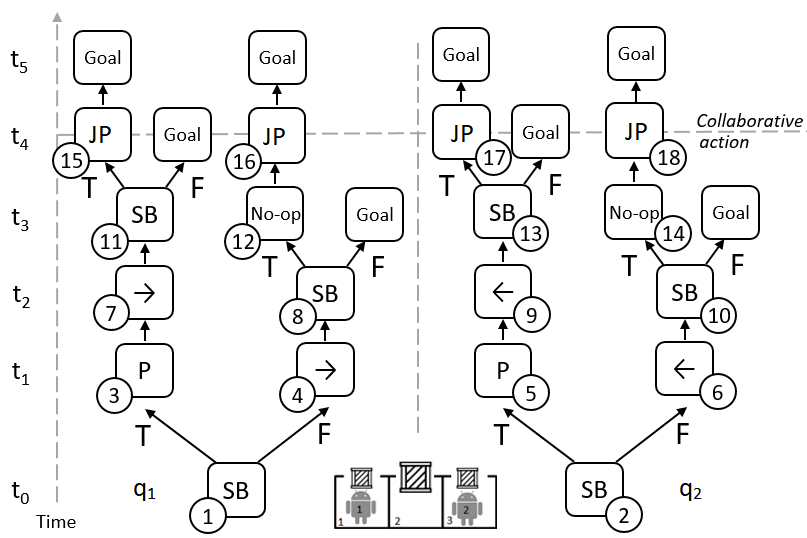
\includegraphics[width=3.3in]{LocalTrees.png}
%\vspace{-12pt}
\caption{\emph{SB} denotes sensing box, arrows denote motion, {\em P} denotes push,
and \emph{JP} denotes joint-push. 
%for showing the box pushing domain with 2 agents and a possible set of local plan trees that produce a solution. Possible agent actions are sensing a box at the current agent location (denoted $SB$), moving (denoted by arrows), pushing a light box up alone (denoted $P$), jointly pushing a heavy box (denoted $JP$), and no-op.
}
\label{fig:LocalTrees}
\end{figure}


%%%%% [SZ] \ \\[-42pt]
\begin{example}
\label{ex:BoxPushing}
%% not sure why figure reference not working? replaced with 1 by Shlomo:
%We now illustrate the factored QDec model using a simple box pushing domain (Figure~\ref{fig:LocalTrees}).
We have a 1D grid of size 3, with cells marked 1-3. The two agents $\varphi_1$ and $\varphi_2$ start in cells 1 and 3. Each cell may contain a box that needs to be pushed upwards. The left and right boxes are light and can be pushed
by a single agent. The middle box is heavy and can
be pushed by two agents acting together. Thus,
$P=\{\mathit{AgentAt}_{i,pos},\mathit{BoxAt}_{j,pos},\mathit{Heavy}_{j}\}$ where $pos \in \{1,2,3\}$ is a grid position, $i \in \{\varphi_1,\varphi_2\}$, and $j \in \{1,2,3\}$ is a box index. In the initial state each box may be in or out of the grid --- $b_0=\mathit{AgentAt}_{\varphi_1,1} \wedge \mathit{AgentAt}_{\varphi_2,3} \bigwedge_{j=1,2,3} (BoxAt_{j,j} \vee \neg BoxAt_{j,j})$. There are therefore 8 possible initial states.

Agents can move left and right, push a light box up, or jointly push a heavy box up. There are no preconditions for moving left and right. The agent must be
in the same cell as the box to push it.
%, i.e. $\mathit{Pre(Left)}=\mathit{Pre(Right)}=\phi$. 
%\guy{We mark here agents using $\varphi$, but above we denoted agents with indexes and later with $a_1$ - check for consistency. I prefer $\varphi_i$ for agents.} \shashank{updated the document throughout with $\varphi$'s}
%For $\varphi$ to push up a box $j$, $\varphi$ must be in the same place as the box. %That is, $\mathit{Pre(PushUp_{\varphi,j})}=\{\mathit{AgentAt}_{\varphi,j}',\mathit{BoxAt}_{j},\neg\mathit{Heavy}_j\}$. 
%For the collaborative joint push action the precondition is  $\mathit{Pre(JointPush_{j})}=\{\mathit{AgentAt}_{\varphi_1,j},\mathit{AgentAt}_{\varphi_2,j},\mathit{BoxAt}_{j},\mathit{Heavy}_j\}$.
%
%The move actions change an agent's position and are independent of the effects of other agent actions.
%, e.g., $\mathit{Right}_{\varphi}=\{(\mathit{AgentAt}_{\varphi,1},\neg \mathit{AgentAt}_{\varphi,1} \wedge \mathit{AgentAt}_{\varphi,2}), (\mathit{AgentAt}_{\varphi,2}, \neg \mathit{AgentAt}_{\varphi,2} \wedge \mathit{AgentAt}_{\varphi,3})\}$.\\
%The only joint effect is for the \textit{JointPush} action.
%-- $\mathit{Eff}(\mathit{PushUp}_{\varphi,2},a_2)$ where $a_2$ is some other action, are identical to the independent effects of action $a_2$, while $\mathit{Eff}(\mathit{PushUp}_{\varphi_1,2},\mathit{PushUp}_{\varphi_2,2})=\{(\phi,\neg BoxAt_{2,2})\}$, that is, if and only if the 
%If the two agents push the heavy box jointly, it (unconditionally) gets moved out of the grid.
There also actions for sensing for boxes --- $\mathit{SenseBox_{\varphi,j}}$, with precondition $\mathit{Pre(SenseBox_{\varphi,j})}=AgentAt_{\varphi,j}$, no effects, and $\mathit{Obs(SenseBox_{\varphi,j})}=BoxAt_{j,j}$.
The goal is to move all boxes out of the grid, i.e., $\bigwedge_j \neg BoxAt_{j,j}$.

Figure~\ref{fig:LocalTrees} illustrates this domain and a possible solution.
\end{example}

In what follows  {\em projected sub-tree} denotes a tree  obtained from the original policy tree by removing some nodes. When a node $n$ labeled by a non-sensing action is removed, the parent of $n$ becomes the parent of the child of $n$. A node $n$ labeled by a sensing action can only be removed if the two child subtrees of $n$ are identical. In that case, the parent of $n$ becomes the parent of one of the identical subtrees.

%\guy{commenting our for now - it is not totally true} If we have a policy tree containing actions of two types $A$ and $B$, and we want to look at the projected sub-tree containing $A$ nodes only, we can imagine iteratively removing all $B$ nodes, until none are left.




\section{The QDec-FP Algorithm}

QDec-FP~\citep{ShekharBS19} operates in three stages. (1) Generate a team solution. (2) Extend the projection of the team solution for each single agent. (3) Align the single agent plan trees.
In the first step, the MA problem is transformed into a single-agent problem by treating all actions as if executed by the same meta-agent. This meta-agent can apply any agent's action and and it is aware at each stage of the results of all sensing actions. We denote the resulting team plan as $\tau_{team}$.
%This single-agent problem is solved using the CPOR contingent planner~\citep{}, which generates a policy tree as its solution. 

In the second step, from $\tau_{team}$, QDec-FP generates for each agent $\varphi_i$ a projection $\tau_{\varphi_i}$. To obtain $\tau_{\varphi_i}$ we first remove from $\tau_{team}$ all non-sensing actions except those executed by agent $\varphi_i$. Next, we remove all private actions of all agents, leaving only nodes labeled by public actions.
Furthermore, for each action $a$ in $\tau_{\varphi_i}$, we remove all its public preconditions, as they are guaranteed to be supplied by some public action in $\tau_{team}$. 
Finally we remove redundant sensing actions --- observations that do not influence how $\varphi_i$ acts. These are sensing actions where both subtrees below the observation are identical, from the perspective of agent $\varphi_i$. 

An example of a team solution, its projection, and the compacted projection is given in Figure~\ref{fig:projected}.  Figure~\ref{fig:projected}A shows the team solution, containing both private and public actions of the %two 
agents. The team plan assumes shared knowledge.
For example, 
%We can see that, e.g., 
in the left branch, only agent $\varphi_1$ senses for the existence of the heavy box, but then both agents jointly push it. Figure~\ref{fig:projected}B shows the projected tree of $\varphi_1$. Private actions of both agents were removed, but sensing actions of both agents remain,
as no sensing action is redundant. Figure~\ref{fig:projected}C shows the projected tree of $\varphi_2$. The public {\em push} action executed by $\varphi_1$ in the team plan was removed. And since $\varphi_2$ operates identically in both subtrees of the team plan, we remove the sensing action at the root of the team plan. 

\begin{figure*}[h!]
\centering
%\vspace{-2cm}
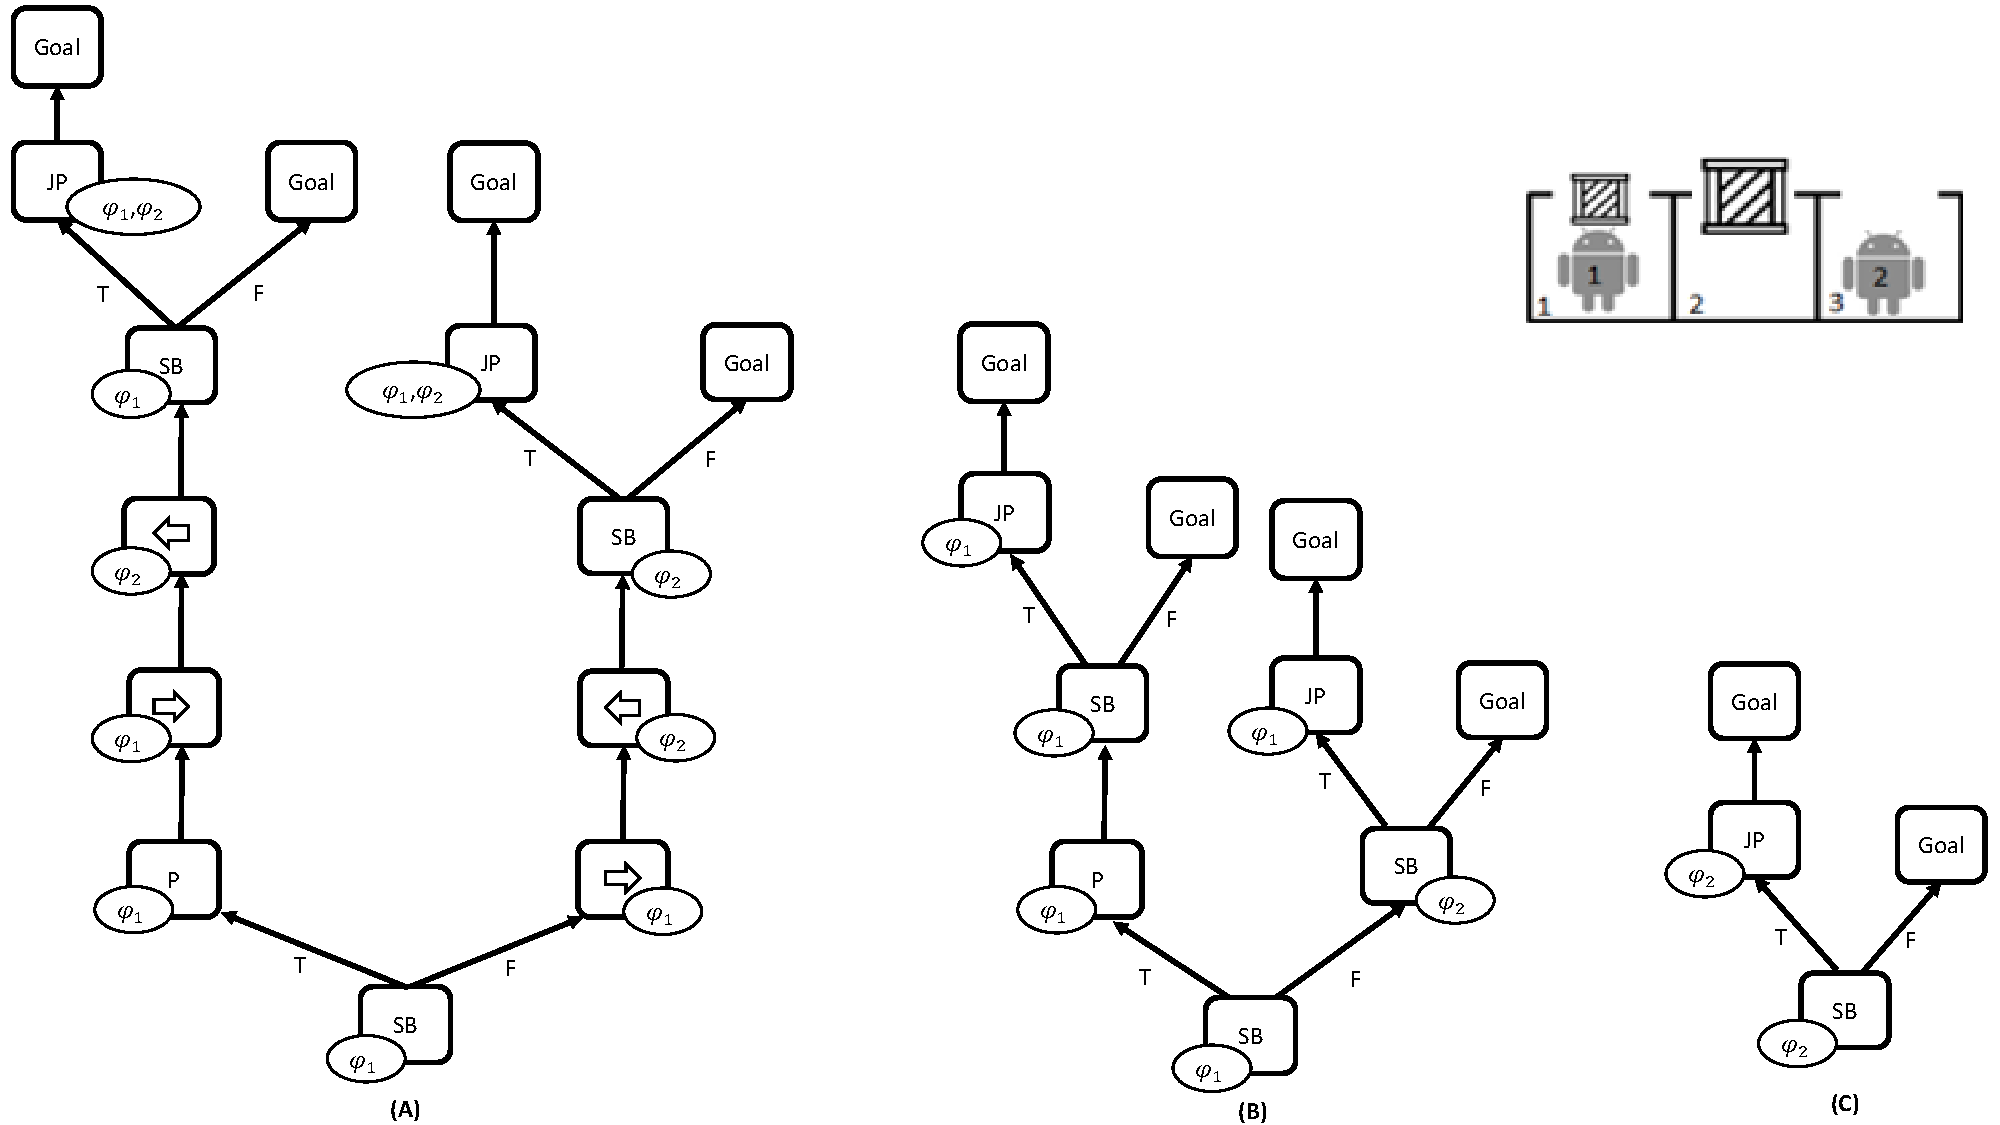
\includegraphics[width=0.8\textwidth, height=2.6in]{main-projection.pdf}
\caption{(A) Team plan tree $\tau_{team}$ for a problem with two agents, a light box and a heavy box that need to be pushed out.
%outside at the edge of the grid in the goal state. 
(B) The projection of $\tau_{team}$ to $\varphi_1$.
%for which all the sensing actions of $\tau_{team}$ are non-redundant.
%and remain. 
(C) A compacted projection for $\varphi_2$.
%in which no sensing action by $\varphi_1$ is required.
}
\label{fig:projected}
\end{figure*}

The projected tree is typically not executable by the agent. It contains sensing actions that are executed by other agents, and some actions require additional preconditions, due to the removal of private actions.
Next, QDec-FP solves a single-agent contingent planning problem for each agent $\varphi_i$ that requires $\varphi_i$ to make $\tau_{\varphi_i}$ executable by adding sensing actions and private actions. 
QDec-FP does not add public actions, as they could interfere with the policies of the other agents by, e.g., consuming a precondition that is needed.  

If some $\tau_{\varphi_i}$ is not solvable, QDec-FP backtracks and seeks a new team solution.
If all $\tau_{\varphi_i}$ are solvable, we know that there is a solution, and all that remains is to align the different policies to ensure that agent actions are executed in the right order -- as reflected by the team policy. This is done by inserting $noop$ actions to postpone actions as need to be.

To implement QDec-FP,
one needs a single-agent off-line contingent planner. 
%, i.e., a contingent planner that generates complete policies. 
QDec-FP uses CPOR~\citep{CPOR}, which generates a policy tree by repeatedly calling the online contingent planner SDR~\citep{SDR}. SDR generates a single execution branch that corresponds to the true initial state. CPOR
simply calls it multiple times with different "true" initial states.
%In the case of CPOR, a different ``true'' initial state is selected by the algorithm until all states have been covered. 

While CPOR is the most scalable offline contingent planner currently, it has a major weakness: it does not backtrack. 
To overcome this, QDec-FP introduced a backtracking mechanism on top of CPOR. It modifies the planning problem with an additional, sound, constraint, that invalidates
previous solutions. 
However, this limits the number of backtracks that are practically possible. 
%
%In addition, the underlying SDR planner performs some limited form of reasoning about the agent's knowledge and uses a regression mechanism to ensure that an action is never executed if its preconditions are not known to hold. Since the regression mechanism is sound, so are the actions selected by SDR.

%The reliance on an online solver that focuses on one branch at a time has important implications for the QDec-FP implementation. 
%The SDR solver is not aware of the choices made in alternative branches. This can lead to a subtle issue when reasoning about the knowledge of different agents, as we later discuss in the case of signaling.

% \shashank{Will fit them soon...}
% \begin{figure}[ht]
%   \subfloat[Team plan]{
% 	\begin{minipage}[c][1\width]{
% 	   0.3\textwidth}
% 	   \centering
% 	   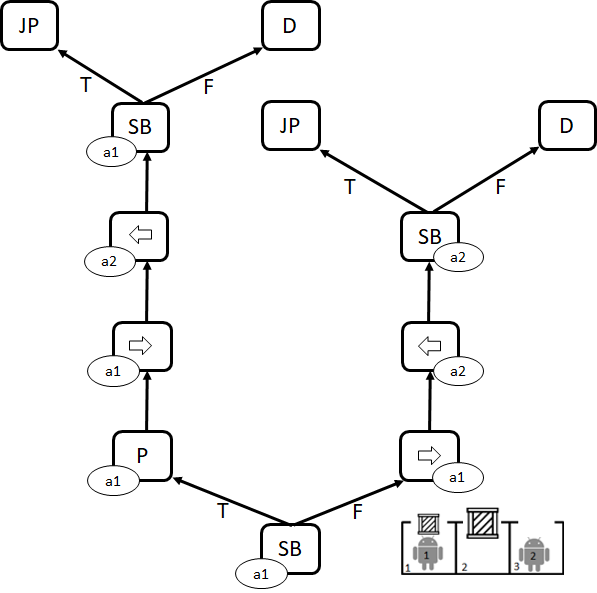
\includegraphics[width=1\textwidth]{team-plan.png}
% 	\end{minipage}}
%  \hfill 	
%   \subfloat[Projection - Agent2]{
% 	\begin{minipage}[c][1\width]{
% 	   0.3\textwidth}
% 	   \centering
% 	   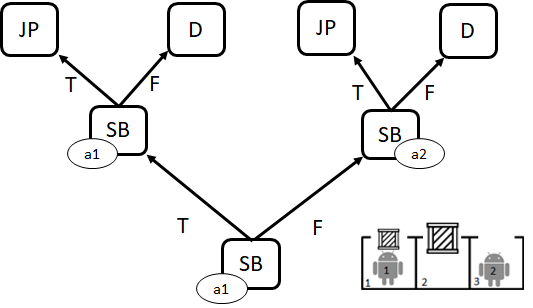
\includegraphics[width=1.1\textwidth]{Proj-Agt2.png}
% 	\end{minipage}}
%  \hfill	
%   \subfloat[Compression]{
% 	\begin{minipage}[c][1\width]{
% 	   0.3\textwidth}
% 	   \centering
% 	   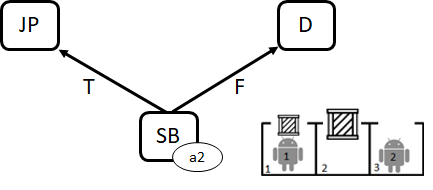
\includegraphics[width=1.2\textwidth]{Proj-Agt2-comp.png}
% 	\end{minipage}}
% \caption{}
% \end{figure}

\section{The QDec-FPS Planner} 
%
%We now describe QDec-FPS.
%(that allows for \emph{Signaling}) planner.
%The 
QDec-FPS 
%algorithm 
has the
same high-level structure as QDec-FP, but modifies the way the team problem is solved, and adds a %pre-processing 
mechanism for generating macros that enable signaling. 
%The use of these macros is needed to overcome the limitations of the underlying CPOR single-agent solver.
%While the ideas underlying this extension --- modeling the knowledge of different agents and the use of signaling --- are general, we also explain the particular technical mechanisms required for integrating these ideas into QDec-FPS.


\subsection{Agent Specific Knowledge}

%\guy{rewriting this section - the beginning with the discussion of sound and complete planners and regression does not seem relevant here}

QDec-FP uses, through the CPOR planner, the SDR translation from contingent planning to classical planning. This translation maintains, for each proposition $p$, two propositions: $Kp$ and $K\neg p$, denoting knowing that $p$ is true or false, respectively.
SDR then transforms each precondition $p$ of an action to $Kp$.
%That is, in addition to requiring that the action will be executable only when $p$ holds, the planner also requires that the agent will {\em know} that $p$ holds. The agent can obtain $Kp$ as a result of a sensing action over the value of $p$.
%
The translation ensures that $Kp$ holds in a belief state only if $p$ holds in all possible worlds.
This is done by reasoning about all the specific possible worlds explicitly. 

The state description in the classical translation contains the current state of the world given every possible initial state, in the form of $Kp|s$, where $p$ is a proposition, and $s$ is a possible state. It also contains actions that allow deducing new knowledge facts, called {\em merge} and {\em refutation} actions~\citep{PalaciosG09}. Thus, the agent can also obtain $Kp$ if for every currently possible state $s$, $Kp|s$ holds.


\commentout{ \guy{Commenting out the below, because it is relevant for the discussion of soundness and completeness, not agent specific knowledge}
If the agent models all possible states of the world, this mechanism is sound, that is, if the planner concludes that $Kp$ holds, then $p$ holds in the current belief state. It is also complete w.r.t.~literals and their conjunction. That is, if $Kp$ holds, the planner can deduce this fact using its inference actions.

Reasoning about the explicit set of possible worlds, which is often exponential, is impractical. Therefore, SDR sub-samples the set of possible worlds, and hence its reasoning is complete, but unsound. CPOR then fixes
this issue by performing regression before inserting any action into its plan, to verify that its preconditions hold in all possible worlds. Because regression is complete, this ensures the overall soundness of the planner. 
}

Because QDec-FP solves the team problem as a single-agent planning problem, the planner treats all agents as part of a single centralized agent, and the knowledge of this agent reflects the combined knowledge of all agents. Thus, when one agent observes that $p$ holds, other agents can use this knowledge, without observing the value of $p$ themselves. This is inconsistent with the real plan tree, where each agent must independently ensure that $p$ holds, before executing an action that requires $p$ as precondition.

QDec-FPS changes SDR's translation to be agent aware. 
The $Kp$ propositions used to capture combined knowledge
are replaced by propositions of the form $K_{\varphi}p$, denoting that agent $\varphi$ knows that $p$ holds. The precondition $p$ of an action executed by agent $\varphi$ is replaced with  $K_{\varphi}p$. The effect of a sensing action executed by $\varphi$ is that only the sensing agent $\varphi$ knows the value of $p$, i.e., either $K_{\varphi}p$ or $K_{\varphi}\neg p$. 
Similarly, merge and refutation actions now provide  agent-specific inference. The effect of a non-sensing action is still known to all agents (as agents are aware of the plan itself).

%\ronen{The main problem here is that this may not be complete. We need to rule out the possibility that an agent knows the value of some proposition not through sensing or signaling, but through additional knowledge implicit in the plan itself. For example, an agent may know, based on the part of the plan it is in now, that some other actions where executed previously, and therefore, some proposition must be true.}
This modification forces the underlying planner to insert sensing actions by different agents to ensure they have the knowledge required to perform their actions, whereas in QDec-FP, because all agents are treated as one, it was enough if some other agent performed this sensing action. If an agent has an action with a precondition $p$, the team plan will ensure that the agent first senses or learns the value of $p$.
If the agent cannot sense or learn the value of $p$, such an action will not be part of a generated team plan.

This leads to the generation of team plans that better account for agent abilities. Like team plans in QDec-FP, these plans may not be extendable because they can require agents to act differently depending on information they do not have. Yet, they are much better informed, and are therefore less likely to lead to failure when agents extend the team plan. Hence, they often lead to fewer backtracks. %This team plan, however, may not be executable in a distributed manner. This is because the team plan may require agents to execute different actions under different branches, among which they cannot differentiate. This requires additional sensing actions, which will be added later.




The new translation also allows us to solve problems that QDec-FP cannot solve. For 
example, imagine
%suppose the values of $p$ and $q$ are always correlated. 
that Agent $\varphi_1$ can observe only $p$, and agent $\varphi_2$ can only observe $q$, but must execute an action with
precondition $p$. QDec-FP's team plan will most likely let $\varphi_1$ sense $p$, and
will make $\varphi_2$ execute the action afterwards. 
%of sensing $p$ by $\varphi_1$ in the team plan. 
This team plan cannot be later extended by $\varphi_2$ to a valid local plan because it cannot sense $p$. QDec-FPS will avoid this team plan because it will know that $\varphi_2$ does not know $p$. Furthermore, as we discuss below, if $\varphi_1$ can set the value of $q$ to be correlated with $p$, it will be able to exploit this implicit form of communication.
%, wand consider team plans where $\varphi_2$ observes $q$, and then reasons about $p$.

%\ronen{Guy - see below}
The new translation is more demanding and generates classical planning problems that are harder to solve.
Because of this, it is able to detect unsolvable problems faster.
However, in the special case of agents with identical capabilities, 
some problems are solved
by QDec-FP while QDec-FPS times-out.
In these problems,  QDec-FP generates a simple team solution that lacks many sensing actions. However, since all agents have identical capabilities, it is easy to add these additional sensing actions
into the projected single-agent planning problems. This simple team solution of QDec-FP is not a legal solution to
the more complex team problem QDec-FPS generates. Solving this more complex problem requires numerous backtracks,
making it unsolvable in the given time.
In a sense, QDec-FP solves a more abstract,
and hence a simpler problem. When most abstract solutions are extendable to full solutions, as in the case of homogeneous agents, this is more efficient for large problems. When the problem's structure is more complicated, as in the case of heterogeneous agents, many solutions to the more abstract problem cannot be extended to a full solution.



\commentout{
\subsection{Agent Specific Knowledge [OLD]}
%%%
A sound contingent plan is one in which an agent never executes an action in a state in which its preconditions may not hold.
SDR, and consequently, CPOR and QDec-FP/S, use two levels of reasoning to ensure both efficient plan generation and soundness.
%our planner has two levels of reasoning that ensure soundness. 
%First, the planning problem that it generates models the set of states each agent considers possible, and consequently, its knowledge, explicitly. However, for efficiency reasons, the model uses only a small sample of these states. While this does not ensure soundness, it does help the planner prune many unsound plans. Then,
%prior to the execution of each action, a complete regression step ensures that the preconditions indeed hold. If they do not, SDR replans.

%regression mechanism that ensures soundness, it relies on a translation to a classical solver to generate plans. 
%To help ensure that these plans are executable, the translated problem contains some epistemic information that models the knowledge of the agent, as well as planning actions that perform simple inference to deduce additional knowledge.
%As explained above, QDec-FP works by calling the CPOR planner, which makes numerous calls to the SDR online contingent planner. 
SDR works by translating the contingent problem into a a classical problem that models the knowledge of the agent. The translation transforms each precondition $p$ of an action to $Kp$, denoting knowing that $p$ holds.
That is, in addition to requiring that the action will be executable only when $p$ is satisfied in the current (assumed) world, the planner also requires that the agent will {\em know} that $p$ holds.
The translation ensures that $Kp$ holds in a belief state only  if $p$ holds in all possible worlds.
This is done by reasoning about all the specific possible worlds explicitly, i.e., the underlying classical planner's state description contains the current state of the world given every possible initial state, and some of its actions allow deducing new knowledge facts (called {\em merge} and {\em refutation} actions~\citep{PalaciosG09}).
If the agent models all possible states of the world, this mechanism is sound. It is also complete w.r.t.~literals and their conjunction. That is, if $Kp$ holds, the planner can deduce this fact using its inference actions.

Reasoning about the explicit set of possible worlds, which is often exponential, is impractical. Therefore, SDR sub-samples the set of possible worlds, and hence its reasoning is complete, but unsound. CPOR then fixes
this issue by performing regression before inserting any action into its plan, to verify that its preconditions hold in all possible worlds. Because regression is complete, this ensures the overall soundness of the planner. 

%Because the number of possible states is exponential, SDR considers only a (small) sample of possible states, which means that an agent's knowledge is over-estimated. Thus, the use of knowledge preconditions prunes many plans that are not sound,
%but it does not guarantee soundness.
%Therefore, on top of this, CPOR uses 
% sound and complete regression mechanism to ensure that the preconditions of any action inserted into the plan hold in all possible worlds.
%\ronen{need to understand if this is true for CPOR.}

Because QDec-FP solves the team problem as a single-agent planning problem, the planner treats all agents as part of a single meta-agent, and the knowledge of this agent reflects the combined knowledge of all agents. 
In QDec-FPS, we replaced the translation that is used by SDR with a new translation that is agent aware. That is, instead of having propositions of the form $Kp$, we have propositions of the form $K_{\varphi}p$, where $\varphi$ is an agent. Now, the precondition $p$ of an action that is executed by agent $\varphi$ is replaced by $K_{\varphi}p$. The effect of a sensing action executed by $\varphi$ is that only the sensing agent $\varphi$ knows the value of $p$, i.e., either $K_{\varphi}p$ or $K_{\varphi}\neg p$. 
The same holds for the merge and refutation actions, which now provide  agent-specific knowledge.

%\ronen{The main problem here is that this may not be complete. We need to rule out the possibility that an agent knows the value of some proposition not through sensing or signaling, but through additional knowledge implicit in the plan itself. For example, an agent may know, based on the part of the plan it is in now, that some other actions where executed previously, and therefore, some proposition must be true.}
This modification forces the underlying planner to insert sensing actions by different agents to ensure they have the knowledge required to perform their actions, whereas in QDec-FP, because all agents are treated as one, it was enough if some other agent performed this sensing action.
On its own, it does not guarantee that the generated team plan is indeed executable, as this team plan may still require agents to execute different actions under different branches among which they cannot differentiate.
However, if an agent has an action with a precondition $p$, the team plan will ensure that the agent first senses or learns the value of $p$.
If the agent cannot sense or learn the value of $p$, such an action will not be part of a generated team plan.

This leads to the generation of much better team plans that better account for agent abilities, and are therefore less likely to lead to a failure in the next stage where each agent extends the team plans. Consequently, it reduces the number of backtracks needed. 

However, as the number of agents increases, it also makes the classical problem generated by SDR larger and more difficult to solve.
In some cases, such problems are solvable by QDec-FP
but not by QDec-FPS.
%In these cases, QDec-FP succeeds because it 
In these latter cases, the situation is usually as follows: the QDec-FP generates a simple team solution that lacks many actions, which are then added when the projected single-agent planning problems are solved.
QDec-FP succeeds here either because this team solution is legal for it, but not for QDec-FPS, or
simply because the classical problem QDec-FPS generates is too hard for the planner.
In a sense, QDec-FP solves a simpler, more abstract problem that ignores some agent specific details, and compensates for it by inserting more actions at the local-agent level, which is relatively easy, too. 
}



\begin{figure*}[h!]
\centering
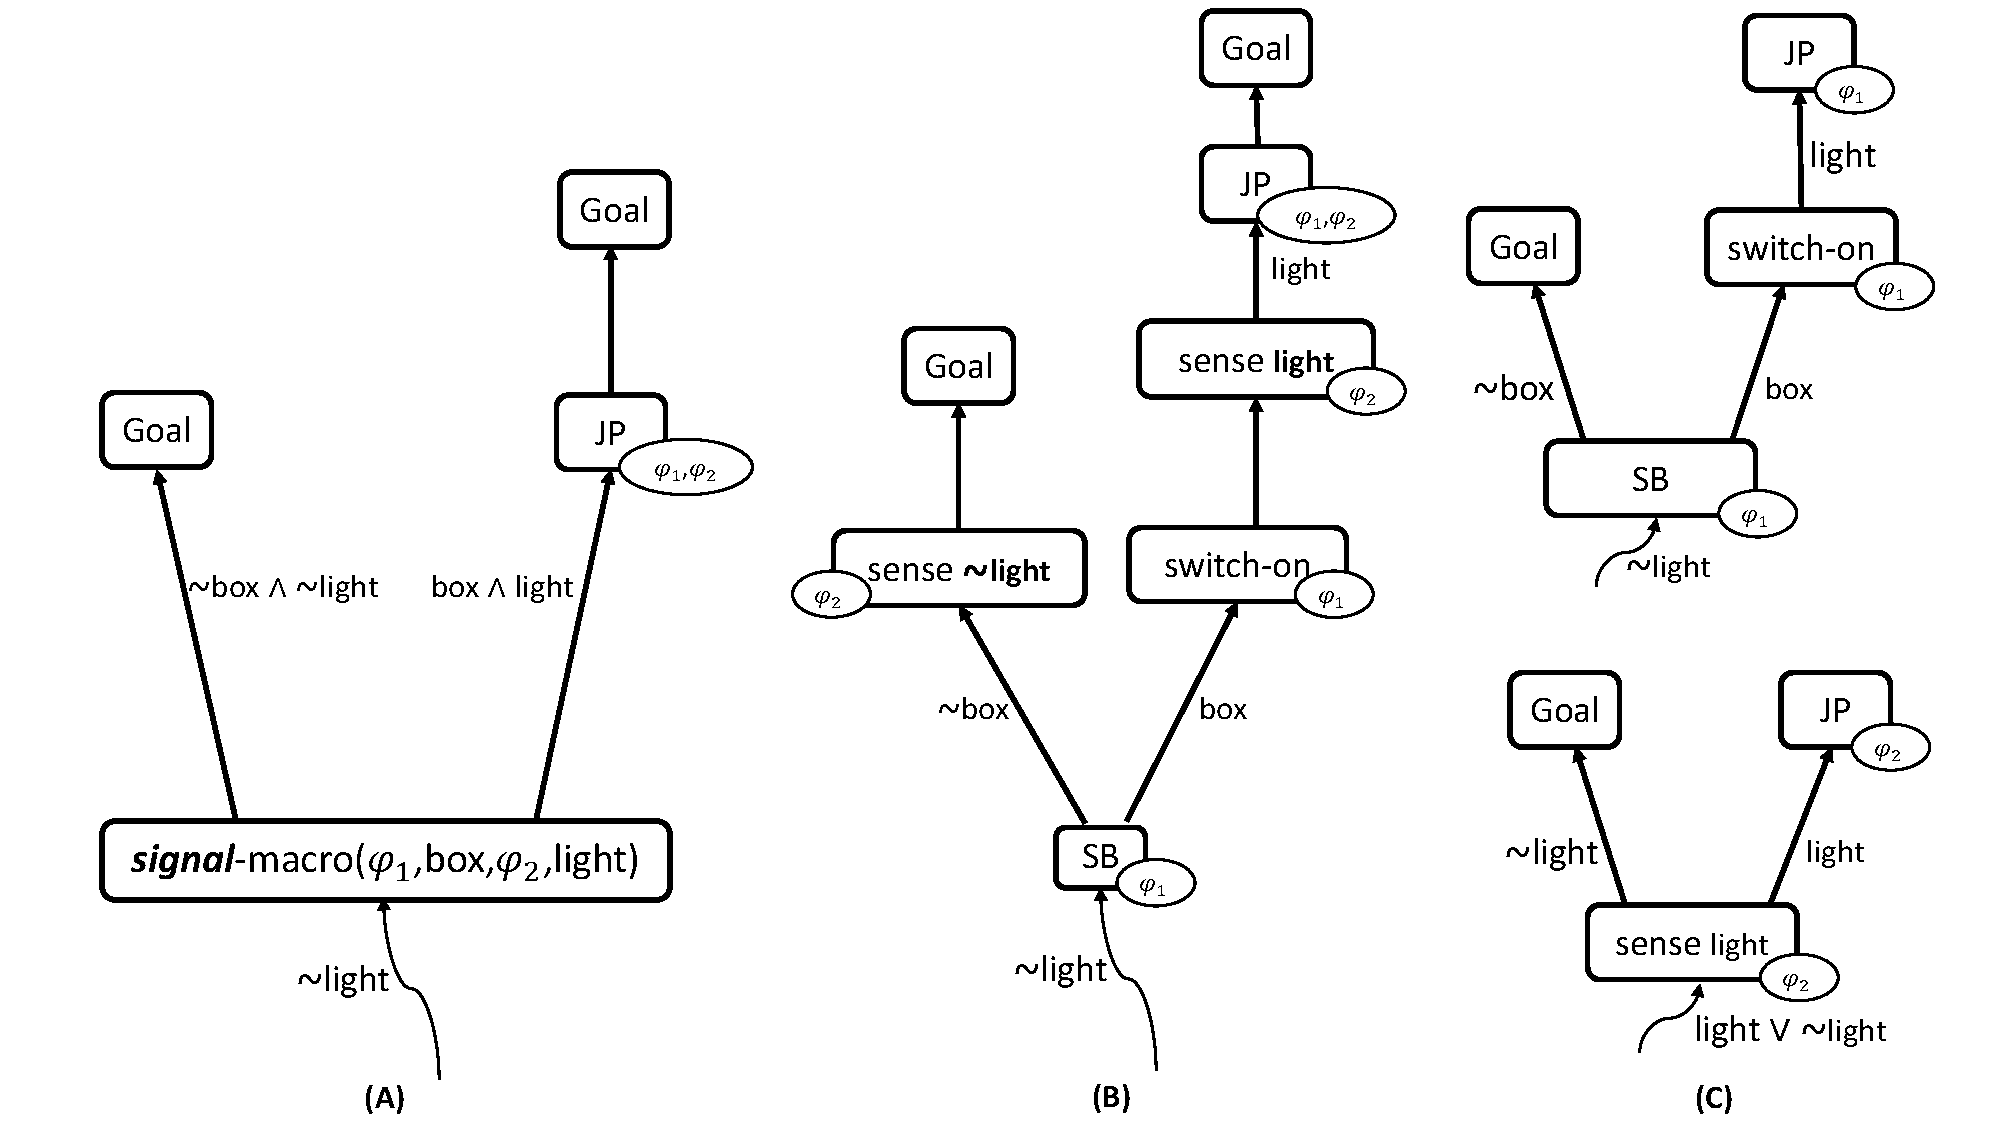
\includegraphics[height=2.6in, width=0.85\textwidth]{signaling-r.pdf}
\caption{
\emph{Signaling} in the QDec-FPS planner. 
(A) A team plan with the signaling macro action.  
(B) The team plan following the macro expansion.
(C) Projected trees for $\varphi_1$ (top) and $\varphi_2$ (bottom).
}
\label{fig:signaling}
\end{figure*}
 
\subsection{Signaling}
\label{subsec:signal}
%\guy{consider moving from $a$ $a'$ to $\varphi_i$ $\varphi_j$}
If agent $\varphi_i$ can sense $p$ but agent $\varphi_j$ cannot, $\varphi_i$ might be able to communicate $p$'s value to $\varphi_j$. 
It could do this directly, if an explicit communication action exists, or indirectly, by setting the value of some variable $q$ that agent $\varphi_j$ can sense, to be correlated with $p$'s value. 
In fact, explicit communication can be viewed as correlating the value of a channel variable with $p$.
Signaling consists of the following steps (1) $\varphi_i$ senses $p$. (2) $\varphi_i$ sets the value of $q$ to the value of $p$. (3)  $\varphi_j$ senses $q$. (4) $\varphi_j$ reasons about the value of $p$.  

Notice that (2) is not a restriction on a single branch of the plan, but a restriction on a sub-tree. $\varphi_i$ must ensure that $p\leftrightarrow q$, which means that it needs to act differently in the
branch where $p$ is true and in the branch where $p$ is false. 

To operationalize this idea, we suggest to model the signaling process as a macro.
In our context, macros are not simply 
a sequence of actions, but rather a sub-tree. 

To construct such macros, we must first discover the possible signaling options. We preprocess the domain seeking quadruples $(\varphi_i, p, \varphi_j, q)$ such that
(1) $\varphi_i$ can sense $p$ but $\varphi_j$ cannot. (2) $\varphi_j$ can sense $q$. 
(3) $\varphi_i$ can modify the value of $q$. 
For simplicity, we consider only propositions $q$ that can be affected by a single action that does not change the value of any other public proposition. This can be extended to more complex sub-plans for modifying the value of $q$.
For each such quadruple, we add the macro-action $signal(\varphi_i, p, \varphi_j, q)$. Notice that this process is problem-instance {\em independent} and can be done in linear time.


The macro $signal(\varphi_i, p, \varphi_j, q)$ is treated by the planner as a sensing action that has two possible outcomes: in one of them $p\wedge q$ holds, and in the other $\neg p\wedge \neg q$ holds. Unlike the pure sensing actions we use, this action changes the state of the world, as well, ensuring that this correspondence between the values of $p$ and $q$ will hold.

Given a team plan with a signaling macro, we first expand the macro as indicated above: First, $\varphi_i$ senses the value of $p$. For each of the two resulting branches, it must ensure that $q$'s value is appropriately correlated, by applying actions that affect $q$'s value appropriately. Then, we add in each branch a sensing action $a_q$ where $\varphi_j$ senses the value $q$. While regular sensing actions have two possible children, $a_q$ has only a single child in the team plan because, at the team level, its outcome is known.
When projected to $\varphi_j$'s local plan, however, $a_q$ appears like a regular sensing action. This macro expansion is described in Figure~\ref{fig:signaling}.



In the next step, the projection of the team plan containing the macro expansion is solved by each agent. This requires, in particular, that agent $\varphi_i$ will change the value of $q$ as needed in each branch, and that both agents perform their sensing actions --- $\varphi_i$ over $p$ and $\varphi_j$ over $q$.

Figure~\ref{fig:signaling} shows an example of this process. Two agents, $\varphi_1$ and $\varphi_2$ must jointly push a heavy box. $\varphi_1$ can sense the box, but $\varphi_2$ can only sense whether a light is on. $\varphi_1$ can  signal to $\varphi_2$ about the box by turning on the light, which is originally off. Figure~\ref{fig:signaling}A shows a team plan with a macro. 
Figure~\ref{fig:signaling}B shows the team plan after macro expansion: $\varphi_1$ senses the box, then turns on the light, if needed, and then $\varphi_2$ senses the light. Finally, both jointly push the box. 
Figure~\ref{fig:signaling}C shows the projected single agent plan trees for $\varphi_1$ and $\varphi_2$.  %$\varphi_2$'s plan contains two children for the {\em sense-light} action, although the team plan does not. This special case is handled in the projection creation for which a time tick (T) is shown in the right (just for a reference).

%One problem with this macro is that it can be executed by agent $\varphi_i$ when it knows the value of $p$. 
%This is not necessarily wrong, but it could lead to an unsound plan. For example, assume that agent $\varphi_i$ is in a branch where it knows that $p$ is \emph{true} and signals by making $q$ \emph{true}. 
%Suppose that in the branch where $p$ is \emph{false}, $q$ can also be \emph{true}. 
%Now, if $\varphi_j$ senses that $q$ is \emph{true}, it cannot conclude that $p$ is \emph{true}, as $\varphi_j$ does not know in which branch $\varphi_i$ is.

%This example illustrates that for signaling to achieve its goal, the correspondence between the two propositions' values must hold in both branches.

%\ronen{Shashank - I think I'm missing something in the description.}
%\shashank{verify.}
In practice, adding this macro on top of an online contingent solver that focuses on a single branch at a time, such as SDR, is not straightforward. To address this, we do the following:
We add an action by $\varphi_i$ that can be viewed as a commitment to ensure that $p\leftrightarrow q$ holds. This action is constrained to be followed immediately by the action of sensing $p$ by $\varphi_i$.
At this point, in the team plan, if agent $\varphi_j$ needs to know the value of $p$, it can use the fact that $p\leftrightarrow q$ to deduce it from the value $q$. To ensure that it learns the value of $p$, we force the action of sensing $q$ in both branches. 
As above, the team plan is post-processed to ensure that $\varphi_i$ does indeed ensure the validity of $p\leftrightarrow q$ following the sensing action. 
%\shashank{Very technical but do we need to mention that even with this approach SDR leads CPOR sometimes to a dead-end, consequently, disables the QDec-FPS? Since it is evident from the experiments ...}
%\ronen{We need to discuss this}

%The commitment to ensure 
%the action
%Because SDR does not have a mechanism for affecting the result of one branch when
%generating another, we must ensure that the signaling macro occurs before $\varphi_i$ branches on the value of $p$. 
%This can be done by requiring that $p$'s value is not known prior to the signaling action.
%We achieve this by ensuring that the translation of the \emph{signal} action has $\neg K_{\varphi_i}p \land \neg K_{\varphi_i} \neg p$ as a precondition.

%\guy{The sentence below is not needed - why discuss equivalent alternatives? This only makes the discussion more muddy.}
%Alternatively, we can force this by adding suitable effects and preconditions to sensing and signaling actions, so that we cannot add the macro for signaling $p$ if $p$ was sensed earlier.


\commentout{
\subsection{Backtracking}
\guy{this is a very minor improvement, consider removing if we lack space}

Not all team solutions correspond to truly distributed solutions that are executable by the agents. More specifically, as CPOR treats the team plan as a single agent problem, it may create plans where an agent $\varphi$ may need to perform different action in two branches, that $\varphi$ does not have a sensing action to distinguish between. 
The enhanced encoding of knowledge leads to much better performance of the planner, requiring fewer, and often no backups on problems solved by QDec-FP. However, backtracks are still required on larger and more difficult problems.

In principle, with a backtracking mechanism for the single-agent contingent solver, we could generate new team solutions until we find one that can be extended to a fully distributed solution. 
Unfortunately, CPOR, which is the only off-line contingent solver that can scale to the problems that we are solving, does not have such a mechanism. 
QDec-FP overcame this by identifying the failure in the team plan and adding a constraint to the team planning problem that makes the generation of this plan impossible. 
That is, QDec-FP adds constraints that make previously generated failed plans non-solutions.

%The team plan fails when it requires the agent to act differently based on information it cannot sense.
%For example, suppose that the agent needs to perform action $a$ if $p$ is {\em true} and a \emph{noop} otherwise, and agent cannot sense $p$. 
%In that case, we add a constraint to the planning problem that requires the agent to either do $a$ under both branches, or not do $a$ at all. 
%Note that, in principle, this constraint can be added from the onset. 
%However, there are many such constraints and their encoding in the planning problem makes it more complex. 
%Hence, QDec-FP takes a lazy approach and adds the constraint only if a plan that violates it was generated. 
%
%%\textbf{MORE INFORMATION ON THE EXACT TECHNIQUE TO BE ADDED}
%---SHASHANK--- $\big \downarrow$

We now briefly review the backtracking technique addressed in Shekhar, Brafman, and Shani~(\citeyear{ShekharBS19}), and then explain an enhancement in QDec-FPS.
For a given team plan, suppose we have an asymmetric sub-tree rooted at an observation of $p$ such that an action $a$ appears in one branch following the observation, but not in the other branch.  If the agent that performs $a$ cannot differentiate between these branches
this plan is not executable and hence QDec-FP needs to backtrack. 
In the next iteration we would add a constraint that forces $a$ to appear either in both branches, or not to appear at all. 
We add a synthetic action {\em commit-$p$} that can only appear before an agent can sense $p$. 
This action has a special effect that is added as a precondition to $a$. 
Thus, if $p$ was observed, $a$ cannot be executed unless, {\em commit-$p$} was executed earlier.  Given
that {\em commit-$p$} was executed earlier,  $a$ must appear in all branches following the observation because
it reinstates a goal condition that {\em commit-$p$} deletes.
With this constraint, we guarantee that the current team plan will not be regenerated.

QDec-FPS has a somewhat stronger mechanism that can handle more complex cases. 
%\guy{again, I suggest moving from $a$ for agent to $\varphi_i$ - this will avoid similar notations for agents and actions}
Suppose that the team plan requires agent $\varphi_i$ to perform action $a_1$ followed by action $a_2$ when $p$ is {\em true} and $a_2$ followed by $a_1$ when $p$ is {\em false}, but agent $\varphi_i$ cannot observe $p$. 
Agent $\varphi_i$ can still preform the actions in a different order even with the new translation (which requires knowledge of action preconditions) if neither $a_1$ nor $a_2$ has $p$ as a precondition. 
Such a policy is not executable by $\varphi_i$ because it cannot distinguish between the two cases. 
However, the backtracking constraint of QDec-FP is insufficient, as it does not enforce action order, only that both $a_1$ and $a_2$ are executed in both branches. 
Instead, we add a similar constraint that allows us to force that not only a single action occurs under both values of $p$, but also that a specific branch will occur under both values of $p$. 
The technical details are similar to the above, where additional propositions are used to enforce the ordering.
}
%
%Suppose that there is a case where an agent, which cannot observe $p$ but, it has to perform both actions $a_1$ and $a_2$ in both the branches under $p$, but they appear in different orders. 
%We note that they are two distinct branches under $p$. 
%Therefore we suggest that one of the most distinct branches should be constrained under $p$. 
%We constrain a branch using an adaptation of the approach explained in the last paragraph. 
%We need extra \emph{synthetic} actions and \emph{propositions} to make sure that $a_1$ and $a_2$ appears in all the branches under $p$ in exactly same order, or they do not not appear at all. 

%In another scenario, suppose that agent $a$ needs to extend its projected solution having different subtrees under $p$ and $a$ cannot sense $p$.
%Following the approach addressed in Shekhar, Brafman, and Shani~[\citeyear{ShekharBS19}], which means if we assume a subtree under $p$ as an \emph{action}, 
%we can constrain it in a similar way a regular action is constrained under an observation variable.
%We can enforce \emph{action} (the subtree) to occur in all the branches rooted at $p$ or not to occur at all.
%However, this can cause QDec-FPS to be incomplete if the selected subtree contain an observation action that belongs to $a'$ \emph{s.t.} $a' \neq a$.
%Hence even in this case too we select a branch of the selected subtree to constrain.
%\ronen{don't understand the last sentence}
%\shashank{rephrased}

%\ronen{I think we need to remove this section for space constraints}
\subsubsection{QDec-FPS Properties.} 
When discussing soundness and completeness, we should first
distinguish between the abstract approach used by QDec-FP/S, which reduces multi-agent contingent planning to single-agent contingent planning, and the practical implementation of the planner which uses a specific planner, CPOR.

First, consider the abstract formulation and assume a sound and complete underlying single-agent contingent planner. The soundness of QDec-FPS without signaling follows from that of QDec-FP: Every team solution of QDec-FPS is also a possible team-solution for QDec-FP and all the other steps are identical. This remains true in the implementation due to the soundness of CPOR. 

With signaling, the abstract version of the macro is a sensing action with effects.
It remains sound if the action used by the signaling agent to ensure that $p\leftrightarrow q$ holds does not affect any other proposition. The implementation using CPOR is more complex, but it ensures that following the commitment to the signaling macro, the team solution implements a correct version of the macro, and hence it is sound, too. 

In the case of completeness, for QDec-FPS, one cannot
separate between an abstract and implemented case because the core contribution of QDec-FPS is at the level of
the implementation of the classical encoding used by CPOR and SDR. At this level, QDec-FPS is incomplete for two
reasons: First, CPOR is an incomplete solver: it lacks an internal backtracking mechanism. (For that reason, the implementation of QDec-FP is also incomplete, although the abstract formulation is complete.)
%\footnote{For that reason, the implementation of QDec-FP is also incomplete, although the abstract formulation is complete. 
%Note that team plans that contain signaling are
%legal team plans for QDec-FP, and thus in theory, do not impact its completeness. In practice, however, such plans are extremely unlikely to be generated.}
Second, the planner's ability to reason about the knowledge of separate agents, as implemented at present, is incomplete. That is, it can under-estimate the knowledge of an agent. Thus, it might not be able to deduce that the preconditions of some actions are known to the acting agent, even though they are. 
%This leads to another source of incompleteness.  



%But assuming a contingent solver that is able to enumerate solutions, instead, a similar completeness argument to QDec-FP holds. We note that signaling does not make the planner theoretically more powerful, in that case, but it does make it more powerful in practice.


\commentout{
\subsection{QDec-FPS Properties}
We now discuss the soundness and completeness of 
QDec-FPS. We rely on results for QDec-FP~\citep{ShekharBS19}.

A sound contingent plan is one in which an agent never executes an action in a state in which its preconditions may not hold.
SDR, and consequently, CPOR and QDec-FP/S, use two levels of reasoning to ensure both efficient plan generation and soundness.
First, the SDR translation requires that an action is executed only if the preconditions of the action are known to hold. However, reasoning about the explicit set of possible worlds, which is often exponential, is often impractical. Therefore, SDR sub-samples the set of possible worlds, and hence its reasoning is complete, but unsound. CPOR then fixes
this issue by performing regression before inserting any action into its plan, to verify that its preconditions hold in all possible worlds. Because regression is complete, this ensures the overall soundness of the planner. 


\noindent{\bf Soundness w/o signaling:} 
 At the level of the team plan, an action $a$ is inserted only if the regression step succeeds. Due to the soundness of regression, the preconditions of $a$ are implied by the initial belief state, the actions carried out, and the observations. In QDec-FPS we regress through the entire set of actions executed by all agents, but the observations of the acting agent only, ignoring observations of other agents. Thus, underestimating the team's knowledge at this branch. From the soundness proof of QDec-FP, we know that if the team plan is sound, then the plan returned after the single-agent planning problems are solved must also be sound.
 
\noindent{\bf Soundness with signaling:} 
The addition of a macro cannot impact soundness, as long as the macro's representation as a single-action reflects the precise effect of its implementation. As described, the macro ensures that $p$ is sensed first, then a single public action affecting the value of $q$ only is allowed, and then $q$ is sensed by the second agent. 
It is not difficult to see that at the end of the process, $p$ and $q$ are correlated, both agents know their values, and no other variable is impacted. 
In the process, no other public variable except for $q$ is impacted. When the local plans are generated, no public propositions are impacted, as in QDec-FP.


\noindent{\bf Completeness:} 
QDec-FPS is incomplete due to CPOR lack of backtracking mechanism. Thus, this proof is under the assumption that we have a mechanism to generate all
plans that a complete offline contingent planner can generate. For this, it is sufficient to show that given a legal multi-agent (MA) plan $\pi$ for our problem, the contingent planner would be able to generate it. Such an MA plan (i.e., the joint-policy) is a legal team plan because any legal MA plan is a legal team plan. We want to show that it could be generated by the contingent planner with the new translation. 

In principle, SDR's translation, if used with all possible initial states could not rule out any action in $\pi$ because all actions are executed when the agent knows their precondition, and the inference actions used by SDR are complete. 
SDR over-approximates the knowledge by ignoring some of the possible states, but over approximation does not rule out legal solutions. The regression step, too, is sound and complete, as the agent can only rely on actions it knows others have executed, its actions, and its observations. 
Note that the agent does not necessarily know what actions other agents have executed because it is not sure on which global execution branch it is within $\pi$. Thus, per-branch, SDR also over-approximates the knowledge of the agent. 
This implies that $\pi$ can be generated as a team plan. 
For the single agent plan trees projected from $\pi$ --- the agent's actions in $\pi$ are a possible solution to the single-agent projected problems.%

This may seem to contradict the soundness. But note two things. (1) In the soundness proof we only wanted to show that the team plan is legal.
Here, we have a full, MA plan. (2) As an agent must execute the same action
in all branches that are indistinguishable, this means that the regression of
the preconditions would return true under all branches, if $\pi$ is a legal multi-agent plan.

Signaling does not impact this result. Signaling is a technique that allows us to generate additional solutions. In principle, a solution with signaling is compatible with the algorithm used without signaling, but a vanilla contingent planner that generates all possible plans will take a long time to accidentally stumble upon a solution that contain signaling. 

We note that, in practice, to make signaling work efficiently, we restrict its application contexts using preconditions that require certain lack of knowledge by the signaling agent, even though this is
not necessary by the theory.
}
%As with the original QDec-FP, QDec-FPS is complete provided that we have a complete underlying single-agent solver. We need to claim that eventually, QDec-FPS will generate a solution. For this we need to bound the number of plans that it can generate, i.e., the number of needed backtracks. Since the constraints we add are weak, it is not clear that we can capture all the possible information, and it may be the case that the planner will always generate illegal solutions.
%Soundness: This should follow from the single-agent soundness of the team problem together with the correct ex- tension by the agents to a MA plan.


% \section{Empirical Evaluation [OLD]}

% We provide an empirical analysis showing the scalability and applicability of our new approach. 
% We compare our current approach (QDec-FPS) with the Factored Planning (QDec-FP) approach. Both planners, QDec-FP and QDec-FPS, are  implemented in C\#, and were run on a Windows 10, 64 bit machine with i7 processor, 2.8GHz CPU, and 16Gb RAM.
% IMAP was excluded as QDec-FP was already shown to scale better than IMAP~\citep{ShekharBS19}.


% \subsection{Domain Description}

% We run the experiments on two domains --- \emph{box-pushing} and \emph{table-mover} --- which we now describe.

% \paragraph{Box-Pushing (BP):}
% There are boxes situated in a grid-like structure. 
% Each box is supposed to moved to its destination location, in this case at the edge of the grid, i.e., at the end of the column the box appears in. 
% Each box is either at some location in the grid or at the goal location. 
% An agent needs to be in the same grid cell where a box exists to observe it and to push it. 
% Boxes are either heavy or light. Two agents are required to push a heavy box successfully, while a single agent can push a light box. 
% Agents can also move between two adjacent locations in the four primary directions. In this domain, we have uncertainty about the initial locations of the boxes.
% The agents are non-homogenous --- different agents can observe and push different boxes.

% \paragraph{Table-Mover (TM):}
% The domain consists of a number of tables and rooms, and agents that can move between connected rooms. 
% The initial location of each table is uncertain, and agents must move each table to its dedicated goal locations. 
% Like the BP domain, agents here are \emph{non-homogeneous} and different agents can sense the location of different tables.
% Each table has some fragile items on top of it, and these objects must remain intact. 
% To achieve this, agent must perform collaborative actions to manipulate the table, for example, collaborative actions like \emph{2move-table}, \emph{2lift-table}, \emph{2drop-table}.
% The actions \emph{2lift-table} and \emph{2drop-table}, indicate that two agents, respectively, lift and drop a table simultaneously, keeping the objects on the table intact in the process. 



% \subsection{Experimental Results}
% %
% We compare the QDec-FPS and QDec-FP approaches on the basis of the policy quality (\emph{max-width}, \emph{max-height}), runtime (\emph{time}), and the number of \emph{backtracks} needed to solve a problem. \emph{max-width} and \emph{max-height} refer to maximum number of branches and the maximum height of all individual solution trees obtained for the agents. The number of branches is also indicative of the number of sensing actions performed, as branching occurs following an observation. The planner backtracks when at least one of the single-agent problems, obtained by decomposing the team solution, is unsolved by CPOR.



% \begin{table}[]
% \centering
% \resizebox{\columnwidth}{!}{%
% \begin{tabular}{c | l | r | r@{}r | r r | r r | r r }
%     \hline \cline{1-11}
% 	\multicolumn{1}{c|}{\multirow{2}{*}{\textbf{Domain}}} & \multicolumn{1}{c|}{\multirow{2}{*}{\textbf{Ins (\#agt)}}} & \multicolumn{1}{c|}{\multirow{2}{*}{\textbf{Objects}}} & \multicolumn{8}{c}{\multirow{1}{*}{\textbf{QDec-FP \emph{vs} QDec-FPS} }} \\
% 	\cline{4-11}
% 	& & & \multicolumn{2}{c|}{\multirow{1}{*}{\emph{Max-Width}}} & \multicolumn{2}{c|}{\multirow{1}{*}{\emph{Max-Height}}} & \multicolumn{2}{c|}{\multirow{1}{*}{\emph{Time (sec)}}} & \multicolumn{2}{c}{\multirow{1}{*}{\emph{BT}}} \\
%     	\hline \cline{1-11}
% 	\multicolumn{1}{c|}{\multirow{15}{*}{\textbf{BP}}} 	
% 											& B1 (3) &16	&8		&5	&23	&18	&3.59		&\textbf{2.91} 	&0		&0 \\
% 										  	& B2 (3) & 12	& 6	& 8	& 16	& 15	& 13.65	& \textbf{2.9}	& 4	& 0 \\
% 											& B3 (3) & 11	& 4	& 4	& 14	& 11	& 16.39	& \textbf{1.17}	& 9	& 0 \\
% 											& B4 (3) & 12	& -		& 6	&	- 	& 12	& - 		& \textbf{13.58}	& {47}$^{\tiny +}$ 	& 4 \\
% 											& B5 (3) & 12	& 8	& 8	& 18	& 19	& 158.89 & 	\textbf{3.87}	& 41	& 0 \\
% 											& B6 (3) & 12	& 8	& 8	& 17	& 21	& 111.6	& \textbf{4.05}	& 26	& 0 \\
% 											& B7 (3) & 13	& 16	& 14	& 21	& 19	& 121.42 & 	\textbf{5.6}	& 19	& 0 \\
% 											& B8 (3) & 16	& 16	& 15	& 26	& 29	& 155.83 & 	\textbf{9.69}	& 33	& 0 \\
% 											& B9 (5) & 20	& * & 24	& *	& 32	& *	& \textbf{75.21}	& *	& 1 \\
% 											& B10 (5) & 20	& * & 24	& *	& 37	& *	& \textbf{365.9}	& *	& 6 \\ \vspace{0.04in}
% 											& B11 (9) & 36	& 64 & *	& 24	& *	& \textbf{25.3}	& *	& 0 & * \\
% 											& B12 (2) & 12	& \emph{na}	& 2	& \emph{na}	& 2	& \emph{na}	& 1.2	& \emph{na}	& 1 \\
% 											& B13 (3) & 13	& \emph{na}	& 4	& \emph{na}	& 7	& \emph{na}	& 5.5	& \emph{na}	& 1 \\
% 											& B14 (3) & 13	& \emph{na}	& 4	& \emph{na}	& 6	& \emph{na}	& 8.9	& \emph{na}	& 2 \\
% 											& B15 (4) & 15	& \emph{na}	& 8	& \emph{na}	& 14	& \emph{na}	& 17.6	& \emph{na}	& 2 \\							

%     	\hline \cline{1-11}
% 	\multicolumn{1}{c|}{\multirow{15}{*}{\textbf{TM}}} 	
% 											& T1 (3) & 8	& 2	& 2	&8	&8	& 11.01 	& \textbf{0.61}	& 7	& 0 \\
% 										  	& T2 (3) & 10 	&8	&7	&20	&16	&\textbf{2.68}	&2.78	&0	&0  \\
% 											& T3 (3) & 10 	&8	&7	&20	&16	&\textbf{34.5}	&41.8	&8	&8  \\
% 											& T4 (3) & 10 	&8	&8	&24	&22	&37.87	&\textbf{22.45}	&9	&4  \\
% 											& T5 (3) & 10 	&-	&-	&-	&-	&140.32	&\textbf{29.73}		&31	&6  \\
% 											& T6 (4) & 12 	&16	&13	&21	&17	&\textbf{7.84}	&8.26 &0 &0  \\
% 											& T7 (4) & 12 	&16	&16	&23	&22	&\textbf{6.68}	&152.18	&0	&14  \\
% 											& T8 (4) & 15 	&12	&16	&34	&26	&\textbf{8.74}	&12.39		&0	&0  \\
% 											& T9 (5) & 14 	&19	&22	&22	&24	&\textbf{20.5} &43.58	&0	&0 \\
% 											& T10 (5) & 16	&12	&14	&32	&25	&\textbf{9.7}		&11.2	&0	&0 \\ \vspace{0.04in}
% 											& T11 (5) & 16	&16	&16	&30	&35	&274.5		&\textbf{56.15}		&27	&3 \\ 
% 											& T12 (2) & 10	& \emph{na}	& 2		& \emph{na}	& 9		& \emph{na}	& 1.7	& \emph{na}	& 0 \\
% 											& T13 (3) & 12 	&2		&2		&16	&11	& 17.59	& \textbf{2.32}	& 9		&0 \\
% 											& T14 (2) & 12 	&\emph{na}	&4		&\emph{na}	&17	& \emph{na}	& 6.81	& \emph{na}		&0 \\
% 											& T15 (3) & 12 	&\emph{na}	&4		&\emph{na}	&19	& \emph{na}	& 11.68	& \emph{na}		&1 \\
%     		\hline 
% \end{tabular}
% }
% \caption{
% %\guy{bold best approach in each row and category}
% Performance comparison of QDec-FP and QDec-FPS planners. 
% \emph{Ins (\#agt)} is instance number with the number of acting agents in the brackets. 
% \emph{Object} denotes the number of objects considered in each problem. 
% \emph{Time} is in seconds. 
% The last column (\emph{BT}) is for number of times a planner backtracks to solve a problem. 
% \textbf{*} is \emph{time out}, '\textbf{-}' represents the planner could not solve it, and \emph{na} is for a problem not applicable to a solver.
% The best approach is shown in \textbf{bold}, selected solely on the basis of \textit{time}.
% }
% \label{tbl:results}
% \end{table}


% Table~\ref{tbl:results} shows that QDec-FPS scales much better than QDec-FP when we have \emph{three} to \emph{five} agents.  
% Specifically, the increase in the number of objects had minor impact on running time of QDec-FPS, as opposed to QDec-FP. 
% We see that for many problems QDec-FPS needs to backtrack only a few times compared to QDec-FP, and as a result, QDec-FPS solves the problems much faster. However, as we discussed earlier, an increase in the number of agents has an adverse effect on QDec-FPS planner, making the team plan much harder to solve.
% In fact, for B11, the problem is solvable by QDec-FP, but the new translation makes it non-solvable by QDec-FPS. 
% We note that for the B11, the agents were \emph{homogeneous} and no backtracking was required to solve.

% We again note that the reason for this is the more stringent demands on the solver in the new translation. In this translation, the solver must ensure that each agent attains the knowledge needed to execute its actions, the $K_{\varphi}p$ propositions. 
% Thus, QDec-FP solves a more abstract problem than QDec-FPS, which is easier to solve. The abstract solution provides in some cases sufficient details for extending the skeleton solution to a concrete plan. 
% Recall that the extension phase involves each agent solving a simpler projected problem. QDec-FPS tracks some agent knowledge details as part of the original team problem.
% As we introduce more backtracking constraints, this eventually becomes too hard for QDec-FPS. It is quite possible that with an underlying solver
% that can perform backtracks, the situation would be different.

% % On the other hand, problems B9, B10, and B11 were solved by the QDec-FPS planner but were unsolved by QDec-FP. 
% % They are  similar problems with similar configurations \guy{similar to what? one another?} and we see that QDec-FPS  needs  at most 11 backtracks to find a solution.   
% % The last four problems in the BP domain capture \emph{signaling}+\emph{backtracking}. 
% % \guy{The claim below requires more details - why do we get into a deadend?}
% % \shashank{Maybe the commented paragraph (in section 5.3 Limitations of CPOR) would work as details?}
% % In these problems, CPOR often gets into a deadend due to the way the signaling macro works. Consequently,
% % QDec-FPS is unable to solve problems with more complex configurations and more agents than B12-B15, that require signaling.

% On the other hand, the problems B9 and B10 were solved by the QDec-FPS planner but were unsolved by QDec-FP. 
% The problems are similar to each other (with almost similar configurations) while we see that QDec-FPS needs  extra backtracks to find the solution.   

% In general, initially, we let the QDec-FPS planner solve a problem such that we do not allow an agent to signal anything to other agent(s).
% Therefore, if the planner fails to find a solution (e.g., when there is a solution in which an agent needs to act differently under $p$ such that the agent cannot sense $p$), we enable a signaling flag ({\em SigFlag}) which adds all possible signaling macros to augment the current problem description, while QDec-FPS solves this augmented planning problem from the beginning.

% We enabled {\em SigFlag} for the problems from B12 to B15 in the BP domain. These problems capture both signaling and backtracking cases. 
% For them, we note that QDec-FPS returned no solution found when the {\em SigFlag} was disabled.
% During solving these problems CPOR often gets into a deadend due to the way the signaling macro works. 
% Consequently, QDec-FPS is unable to solve problems with more complex configurations and more agents than problems B12 to B15, when they require signaling. 
% %\guy{The claim requires more details - why do we get into a deadend?}
% %\shashank{Maybe the commented paragraph (in section 5.3 Limitations of CPOR) would work as details?}

% % The bottom half of the table shows the results for the Table-Mover (TM) domain. 
% % We show results on 15 problems involving different configurations with different numbers of agents.
% % TM is more complex compared to the BP domain as the only public actions in TM are collaborative actions~\citep{brafman2008one}. \guy{why is this more complicated than having additional public actions that are not collaborative?}
% % In problems T1 to T11, similar to the BP domain, when backtracking is not required (\guy{better put all problem indexes here, not just e.g.} e.g., T6, T8), QDec-FP requires less time to solve a problem than QDec-FPS. Whenever problems are more complex, and backtracking is required (e.g., T4, T11), QDec-FPS solves the problems much faster as QDec-FPS requires fewer backtracks than QDec-FP.

% % However, this intuition does not hold for T7 \guy{where...}. 
% % The QDec-FPS solver can also be faster in concluding that a problem is unsolvable (problem T5). For T5 QDec-FPS backtracked only 6 time to decide on \guy{unsolvability?}, compared to QDec-FP which backtracked 31 times. This is because fewer solutions are possible for the classical problem generated by QDec-FPS.

% % We run {\em four} problems that \guy{require?} signaling, T12-T15, which are relatively simpler compared T1-T11, with fewer agents. 
% % In T13, there are 3 agents, $a_1$, $a_2$, and $a_3$ such that $a_1$ and $a_3$ together are sufficient to solve this problem without signaling. QDec-FP solved T13 while backtracking \emph{nine} times.
% % As we purposely placed $a_3$ farther from the table's location, QDec-FPS generated a plan where $a_1$ signaled to $a_2$ the table's location and they achieved the goal together, without $a_3$. This solution was generated much quicker and with no backtracks.
% % If we disallow signaling, QDec-FPS still solves this problem with \emph{zero} backtrack, but it takes more time than  when signaling is allowed. 

% %%rewritten
% The bottom half of the table shows the results obtained in the Table-Mover (TM) domain. We show results on 15 problems involving different configurations with different numbers of agents, such that in most of them the agents are heterogeneous in most problems.
% In contrast to the BP domain the TM domain contains each public action as a collaborative action, e.g., {\em 2lift, 2move, 2drop}. 
% %
% %
% Similar to the BP domain, when backtracking is not required to solve a problem, e.g., instances from T6 to T10, the QDec-FP solver takes less time to find a plan tree than the QDec-FPS solver. 
% Whenever problems are more complex such that backtracking is required, e.g., for the instances T4 and T11, QDec-FPS solves them much faster because QDec-FPS requires fewer backtracks than QDec-FP, in general.
% However, this intuition does not hold for the instance T7 as QDec-FPS backtracked 14 times. 

% \guy{I do not understand the discussion below - did you experiment with unsolvable problem instances?}
% The outer loop of Algorithm~1~\citep{ShekharBS19} goes over every possible team solution before it concludes that there is {\em no solution}.
% Due to this reason and as QDec-FPS generates fewer number of team solutions for a problem as of QDec-FP, at times, the QDec-FPS solver can also be faster to conclude that there does not exist any solution for a problem.
% For the instance T5, QDec-FPS backtracked only {\em six} time to decide that there is no solution as compared to the QDec-FP solver which backtracked 31 times. 

% We enabled {\em SigFlag} for the problems from T12 to T15 in the TableMover domain. 
% They are comparatively simpler in configuration than the previous problems with fewer agents. However, problem T13 shows how signaling can affect the overall runtime when a problem can be solved even without signaling and the new translation.
% %
% %We run {\em four} problems that \guy{require?} signaling, T12-T15, which are relatively simpler compared T1-T11, with fewer agents. 
% There are three agents, $\varphi_1$, $\varphi_2$, and $\varphi_3$ such that $\varphi_1$ and $\varphi_3$ together are capable to solve this problem without signaling. QDec-FP solved T13 while it backtracked \emph{nine} times.
% As we purposely placed $\varphi_3$ farther from the table's location, QDec-FPS generated a plan where $\varphi_1$ signaled to $\varphi_2$ the table's location and they achieved the goal together, without $\varphi_3$. This solution was generated much quicker and with no backtracks.
% If we disallow signaling ({\em SigFlag} is disabled), QDec-FPS still solves this problem with \emph{zero} backtrack, but it takes more time than when \emph{SigFlag} is enabled. 

% \commentout{
% \subsection{Limitations of CPOR}

% The underlying planner used in both QDec-FP and QDec-FPS planners is CPOR --- an offline contingent planner that operates by calling the SDR 
% online replanner. 
% SDR takes a contingent planning problem as an input and translates it to a classical planning problem, and solves it using a classical planner.
% The classical problem generated by SDR is based on the assumption that some state $s$,
% sampled from the initial belief state, is the true initial state in the real world.
% SDR executes the solution generated by the classical solver until either the goal was reached
% or a sensing action returns an unexpected result. A result is unexpected if it is not what would have been sensed
% if $s$ was indeed the true initial state. At that point, SDR replans using the new information. 
% %Based on this assumption, Fast-Forward (FF) finds a classical plan. SDR executes it unless, by sensing the actual environment, the plan breaks the made-up assumptions.
% %Eventually SDR refutes that selected state, rectifies the assumptions and replans online by sampling a new state from the current belief state. 
% SDR repeats this process until it reaches the goal.
% Therefore every successful execution from the initial belief to the goal generates a branch of a sound plan tree.  
% CPOR exploits this online replanning technique to generate a complete plan tree considering all possible initial world states as the guessed \emph{true} state.
% CPOR is sound and complete if  the underlying planner is sound and complete.
% %It is also the fastest contingent planner but it suffers a major weakness. 
% However, CPOR cannot handle avoidable deadends as it performs no backtracking.  Sometimes this causes problems to our QDec-FPS planner while handling signaling actions, making QDec-FPS wrongly conclude that a problem is unsolvable. 
% }
% %We illustrated in the previous section that 
% %As we addressed earlier the correspondence between the values of propositions $p$ and $q$ must hold.
% %For that the underlying planner must ensure that the signaling macro occurs before agent $a$ branches on the value of $p$ and is done by a precondition $\neg K_ap \land \neg K_a\neg p$ to the signaling action. 
% %This might lead CPOR to an avoidable deadend. 
% %
% %
% %The following example from the box-pushing domain illustrates a case in which CPOR fails to solve the problem because it enters into an avoidable dead-end. 
% %There are two \emph{non-homogeneous} agents $a_1$ and $a_2$, a box \emph{B} that is initially at either location \emph{loc1} or \emph{loc2}, the goal is \emph{(box-at B loc2)}.   An additional proposition is \emph{light}, which is \emph{false} initially, which can be used for signaling.
% %Suppose that only $a_1$ can sense the box and only $a_2$ can push the box. 
% %%An additional proposition is \emph{light}, which is \emph{false} initially, and can be used by $a_1$ to signal the position of \emph{B} to $a_2$.
% %A legal team plan for this description would be as follows: $a_1$ signals \emph{(box-at B loc1)} to $a_2$ using the light.
% %Recall that our signaling macro had a conditional effect of making {\em light} true if  \emph{(box-at B loc1)} is true.
% %%however its conditional effect hides the \emph{status} of \emph{light}. 
% %Next, \emph{light} is sensed by $a_2$ which leads to two branches. 
% %%$a_2$ regresses and finds out that when \emph{light} is \emph{on} then \emph{(box-at B loc1)} holds, while in the other branch \emph{(not  (box-at B loc1))} holds.
% %%Finally, 
% %If \emph{light}, $a_2$ pushes \emph{B} to the goal, otherwise the goal condition \emph{(box-at B loc2)} already holds. 
% %
% %%Let us consider another scenario. 
% %Suppose that SDR solves this problem under the assumption that \emph{(box-at B loc1)} holds in the initial state. 
% %Then a possible plan is:
% %%Since the heuristic function employed in FF planner is not very informed, it can generate a classical plan as follows: 
% %$a_1$ observes the proposition \emph{(box-at B loc1)}.
% %If \emph{true}, the action \emph{signal($a_1$, (box-at B loc2), $a_2$, light)} is applied, and then after sensing \emph{light}, agent $a_2$ pushes the box from \emph{loc1} to \emph{loc2}. 
% %CPOR uses this classical plan such that with the first observation action, it reaches two different belief states where \emph{(box-at B loc1)} hold when $a_1$ observes \emph{(box-at B loc1)} and \emph{(box-at B loc2)} holds  
% %when it observes \emph{(not (box-at B loc1))}. 
% %In the next iteration, CPOR selects the assumption that \emph{(box-at B loc1)} holds. %such that only $a_1$ has this knowledge.
% %%, i.e., it continues the plan following the sensing action assuming that ?? chooses the former belief state. 
% %At this point, we would like $a_1$ to signal \emph{(box-at B loc1)} to $a_2$ so that $a_2$ can push the box to the goal location. 
% %However, the \emph{signal-p}'s translation requires that $\neg K_ap \land \neg K_a\neg p$ hold, hence the signaling action cannot be applicable as $a_1$ already knows \emph{(box-at B loc1)}.
% %

\begin{table}[ht!]
\centering
\resizebox{\columnwidth}{!}{%
\begin{tabular}{@{}l | l | r | r@{}r | r r | r r | r r@{} }
    \hline \cline{1-11}
	\multicolumn{1}{@{}l|}{\multirow{2}{*}{\textbf{Domain}}} & \multicolumn{1}{c|}{\multirow{2}{*}{\textbf{Ins (\#agt)}}} & \multicolumn{1}{c|}{\multirow{2}{*}{\textbf{Objects}}} & \multicolumn{2}{c}{\multirow{1}{*}{\textbf{Max-width} }} 
	& \multicolumn{2}{c}{\multirow{1}{*}{\textbf{Max-height} }}
	& \multicolumn{2}{c}{\multirow{1}{*}{\textbf{Time (sec)} }} 
	& \multicolumn{2}{c}{\multirow{1}{*}{\textbf{BT} }}\\
	\cline{4-11}
	& & & \emph{fp} & \emph{fps} & \emph{fp} & \emph{fps} & \emph{fp} & \emph{fps} & \emph{fp} & \emph{fps} \\
    	\hline \cline{1-11}
	\multicolumn{1}{@{}l|}{\multirow{16}{*}{\textbf{BP}}} 	
											& B1 (3) &16	&8		&5	&23	&18	&3.59		&\textbf{2.91} 	&0		&0 \\
										& B2 (4) &16	&12		&10	&19	&19	&\textbf{5.3}		&6.1 	&0		&0 \\	
								\vspace{0.02in}
								
							    & B3 (9) & 36	& 64 & *	& 24	& *	& \textbf{25.3}	& *	& 0 & * \\
							    \cdashline{2-11} %\cdashline{2-11} 
											& B4 (3) & 11	& 4	& 4	& 14	& 11	& 16.39	& \textbf{1.17}	& 9	& 0 \\
					
					& B5 (3) & 12	& 6	& 8	& 16	& 15	& 13.65	& \textbf{2.9}	& 4	& 0 \\ 						& B6 (3) & 12	& -		& 6	&	- 	& 12	& - 		& \textbf{13.58}	& {47}$^{\tiny +}$ 	& 4 \\
											& B7 (3) & 12	& 8	& 8	& 18	& 19	& 158.89 & 	\textbf{3.87}	& 41	& 0 \\
											& B8 (3) & 12	& 8	& 8	& 17	& 21	& 111.6	& \textbf{4.05}	& 26	& 0 \\
											& B9 (3) & 13	& 16	& 14	& 21	& 19	& 121.42 & 	\textbf{5.6}	& 19	& 0 \\
											& B10 (3) & 16	& 16	& 15	& 26	& 29	& 155.83 & 	\textbf{9.69}	& 33	& 0 \\
											& B11 (5) & 20	& * & 24	& *	& 32	& *	& \textbf{75.21}	& *	& 1 \\
											\vspace{0.02in}
											& B12 (5) & 20	& * & 24	& *	& 37	& *	& \textbf{365.9}	& *	& 6 \\
											\cdashline{2-11} %\cdashline{2-11}
					& B13 (2) & 10	& \emph{na}	& 2	& \emph{na}	& 6	& \emph{na}	& \textbf{1.06}	& \emph{na}	& 0 
					\\
					
					 & B14 (2) & 12	& \emph{na}	& 2	& \emph{na}	& 2	& \emph{na}	& \textbf{1.20}	& \emph{na}	& 1 \\
					
					& B15 (3) & 12	& \emph{na}	& 4	& \emph{na}	& 12	& \emph{na}	& \textbf{2.49}	& \emph{na}	& 0 \\						& B16 (3) & 13	& \emph{na}	& 4	& \emph{na}	& 7	& \emph{na}	& \textbf{5.5}	& \emph{na}	& 1 \\
											& B17 (3) & 13	& \emph{na}	& 4	& \emph{na}	& 6	& \emph{na}	& \textbf{8.9}	& \emph{na}	& 2 \\
					
					& B18 (3) & 14	& \emph{na}	& 6	& \emph{na}	& 16	& \emph{na}	& \textbf{4.04}	& \emph{na}	& 0 \\
					
					& B19 (4) & 15	& \emph{na}	& 8	& \emph{na}	& 14	& \emph{na}	& \textbf{17.6}	& \emph{na}	& 2 \\							

    	                            \hline \cline{1-11}
	                                    \multicolumn{1}{@{}l|}{\multirow{15}{*}{\textbf{TM}}} 								  	
	                                        & T1 (3) & 10 	&8	&7	&20	&16	&\textbf{2.68}	&2.78	&0	&0  \\
										  	& T2 (4) & 12 	&16	&13	&21	&17	&\textbf{7.84}	&8.26 &0 &0  \\
											& T3 (4) & 15 	&12	&16	&34	&26	&\textbf{8.74}	&12.39		&0	&0  \\
											& T4 (5) & 14 	&19	&22	&22	&24	&\textbf{20.5} &43.58	&0	&0 \\ \vspace{0.02in}			
											
					                        & T5 (5) & 16	&12	&14	&32	&25	&\textbf{9.7}		&11.2	&0	&0 \\
					                    %\cdashline{2-11}
					                    \cdashline{2-11}
						                    & T6 (3) & 8	& 2	& 2	&8	&8	& 11.01 	& \textbf{0.61}	& 7	& 0 \\
						                    & T7 (3) & 10 	&8	&7	&20	&16	&\textbf{34.5}	&41.8	&8	&8  \\
											& T8 (3) & 10 	&8	&8	&24	&22	&37.87	&\textbf{22.45}	&9	&4  \\
											& T9 (3) & 10 	&-	&-	&-	&-	&140.32	&\textbf{29.73}		&31	&6  \\	
											& T10 (4) & 12 	&16	&16	&23	&22	&\textbf{6.68}	&152.18	&0	&14  \\
											\vspace{0.02in}
											& T11 (5) & 16	&16	&16	&30	&35	&274.5		&\textbf{56.15}		&27	&3 \\ 
				                        %\cdashline{2-11}
					                    \cdashline{2-11}							
					                        & T12 (2) & 10	& \emph{na}	& 2		& \emph{na}	& 9		& \emph{na}	& \textbf{1.7}	& \emph{na}	& 0 \\
											& T13 (2) & 12 	&\emph{na}	&4		&\emph{na}	&17	& \emph{na}	& \textbf{6.81}	& \emph{na}		&0 \\
											& T14 (3) & 12 	&2		&2		&16	&11	& 17.59	& \textbf{2.32}	& 9		&0 \\
											& T15 (3) & 13 	&\emph{na}	&4		&\emph{na}	&14	& \emph{na}	& \textbf{7.80}	& \emph{na}		&0 \\
						& T16 (3) & 14  	&\emph{na}	&4		&\emph{na}	&19	& \emph{na}	& \textbf{11.68}	& \emph{na}		&1 \\
    		\hline 
    		\cline{1-11}
	\multicolumn{1}{c|}{\multirow{22}{*}{\textbf{\textcolor{black}{Rovers}}}} 
	& R1 (1) & 12 & 2 & 2	&8	&8	& 3.8 & 3.8 & 0	& 0 \\ 
	& R2 (2) & 14 & 2 & 2	& 9	& 8	& 5.4 	& \textbf{5.3}	& 0	& 0 \\ 
	
	& R3 (2) & 13 & 4 & 4	& 15	& 15	& 9.3 	& \textbf{8.9}	& 0	& 0 
	\\ 
	& R4 (2) & 17   & 12  & 12	& 34	& 23	& \textbf{35.8} 	& 38.6	& 0	& 0
	\\ 
	& R5 (3) & 18	&12	&12	&28	&32	&\textbf{51.5}	&54.1	&0	&0
	\\
	& R6 (3) & 21	&30	&30	&36	&29	&136.6	&\textbf{111.9}	&0	&0
	\\
	& R7 (3) & 23	&98	&81	&50	&45	&567.9	&\textbf{233.2}	&0	&0
	\\
	\cdashline{2-11} 
	%\cdashline{2-11}
	& R8 (3) &13    &2	&2	&7	&6	&57.9	&\textbf{5.9}   &3	&0
	\\
	& R9 (3) &14	&4	&4	&12	&12	&113.8	&\textbf{10.2}	&4	&0
	\\
	& R10 (3) &14	&4	&4	&11	&11	&314.5	&\textbf{89.3}	&11	&3
	\\
	& R11 (3) &19	&-	&12	&-	&12	&325.1	&\textbf{41.1}	&6+	&0
	\\
	& R12 (4) &15	&4	&4	&12	&11	&47.2	&\textbf{16.0}	&1	&0
	\\
	& R13 (4) &20	&12	&12	&25	&19	&241.8	&\textbf{49.1}	&3	&0
	\\
	\cdashline{2-11} 
	%\cdashline{2-11}
	& R14 (2) &16	& \emph{na}	& 2	&\emph{na}	&9	&\emph{na}	&\textbf{3.6}	&\emph{na}	&0
	\\
	& R15 (2) & 18	& \emph{na}	& 2	&\emph{na}	&10	&\emph{na}	&\textbf{5.89}	&\emph{na}	&0
	\\
	& R16 (2) & 16	& \emph{na}	& 4	&\emph{na}	&13	&\emph{na}	& \textbf{34.17}	&\emph{na}	&0
	\\
	& R17 (2) & 20	& \emph{na}	& 4	&\emph{na}	& 14	&\emph{na}	& \textbf{17.68}	&\emph{na}	&0
	\\
	& R18 (3) & 17	& \emph{na}	& 2	&\emph{na}	&7	&\emph{na}	& \textbf{10.17}	&\emph{na}	&0
	\\
	& R19 (3) & 18	& \emph{na}	& 4	&\emph{na}	&13	&\emph{na}	& \textbf{12.93}	&\emph{na}	&0
	\\
	& R19 (3) & 14	& \emph{na}	& 2	&\emph{na}	& 7	&\emph{na}	& \textbf{6.62}	&\emph{na}	&0
	\\
	& R20 (3) & 19	& \emph{na}	& 8	&\emph{na}	&16	&\emph{na}	& \textbf{36.74}	&\emph{na}	&0
	\\
	& R21 (4) & 20	& \emph{na}	& 6	&\emph{na}	&11	&\emph{na}	& \textbf{67.79}	&\emph{na}	&0
	\\
	& R22 (4) & 22	& \emph{na}	& 6	&\emph{na}	&12	&\emph{na}	& \textbf{68.21}	&\emph{na}	&0
	\\
	\hline 
\end{tabular}
}
\caption{ 
Comparison of QDec-FP and QDec-FPS planners. 
\emph{Ins (\#agt)}: instance number and
number of acting agents. 
\emph{Object}: the number of objects in each problem. 
%\emph{Time} is in seconds. 
\emph{BT}: number of planner backtracks.
\textbf{*}: time out. '\textit{-}':  planner could not solve or breaks down.  \emph{na}: problem not applicable to a solver. \emph{fp}: QDec-FP.
\emph{fps}: QDec-FPS. The best approach, based on time only, is shown in bold. 
}
\label{tbl:final-results}
\end{table}

%Table~\ref{tbl:final-results} compares the performance of our QDec-FPS planner with
%QDec-FP.
%These planners are compared on BP and TM domains for which 16 and 15 problems have been shown, respectively. 
%The table is divided in two major part, one for each domain. Within each domain,
%dashed lines separate three problem classes: homogeneous agents,
%non-homogeneous agents, and non-homogeneous agents that require signaling to solve a problem. 


\section{Empirical Evaluation}

We now examine the applicability and scalability of QDec-FPS by comparing it with QDec-FP on 3 multi-agent planning domains.
Some problems in each domain were modified to require \emph{signaling}.
%
Both QDec-FP and QDec-FPS are  implemented in C\#, and were run on a Windows 10, 64 bit machine with \emph{i}7 processor, 2.8GHz CPU, and 16Gb RAM.
IMAP was not considered, as QDec-FP was  shown to scale better than IMAP~\citep{IMAP}.

We experiment with the following three domains:
%\subsection{Domain Description}
%We consider three planning domains.

\noindent{\bf Box-Pushing (BP)}: Boxes located in a grid-like structure. Each box is to be pushed to its destination location
%, in this case at the edge of the grid, i.e., at the end of the column the box appears in. 
outside the column the box appears in \citep{BrafmanSZ13}.
%Each box is either at some location in the grid or at the goal location. 
%An agent needs to be in the same grid cell where a box exists to observe it and to push it. Boxes are either heavy or light. 
A light box can be pushed by a single agent co-located with the box while a heavy box requires two co-located agents. 
%Two agents are required to push a heavy box successfully, while a single agent can push a light box. Agents can also move between two adjacent locations in the four primary directions. In this domain, we have uncertainty about the initial locations of the boxes.
Agents can be non-homogeneous, i.e., different agents can observe and push different boxes.

\noindent{\bf Table-Mover (TM)}: TM consists of a number of tables and rooms, and agents that can move between connected rooms \citep{ShekharB20}. 
The tables' locations are uncertain initially, and agents must move them to their goal locations. 
Agents can be non-homogeneous in their sensing and manipulation abilities.
%where different agents can sense the locations of different tables.
%Each table has some fragile items on top of it, and these objects must remain intact. 
All table manipulation actions are collaborative:
%Agents must perform collaborative actions to manipulate the table, for example, collaborative actions like 
\emph{2move-table}, \emph{2lift-table}, \emph{2drop-table}.
%The actions \emph{2lift-table} and \emph{2drop-table}, indicate that two agents, respectively, lift and drop a table simultaneously~\citep{ShekharB20}.
%, keeping the objects on the table intact in the process. 

\noindent{\bf Rovers}: 
%domain as formulated in the International Planning Competitions (IPCs) is a single-agent domain but it was originally motivated by real multi-agent applications used by NASA.
%It involves 
Multiple rovers navigate a planet surface, finding samples and communicating them back to a lander \citep{IMAP}.
%We adapted this domain to test our QDec-FP and QDec-FPS planners, which is an extension of multi-agent Rovers domain in which multiple rovers (\emph{i.e.}, agents) collect  measurements of a rock sample together, \emph{e.g.}, 
Two rovers must simultaneously collect the rock sample, while a single agent can sample soil as well as take images of certain objectives on its own. 
Coordination points include locations (waypoints) which are accessible to multiple rovers. Rovers communicate sampled soil/image/rock data to the lander that exists at a certain waypoint. 
A rover navigates between two waypoints 
%on the surface and to collect measurements, for which the rover 
and must be present at the corresponding %waypoint 
%where it is allowed 
to sample. 
Availability of data to sample at a waypoint is unknown to the rovers initially. 
%
%A rover at a waypoint can attempt a   measurement, but whether the rover would measure things successfully is actually based on if the waypoint is appropriate for that measurement. 
%
%Samples of soil and rock, and images can be collected by a single rover. 
In this modified domain, our schema requires two rovers working jointly to collect rock samples. After taking measurements, the rovers must broadcast them back to the lander.
In this domain in general, a rover has fewer public actions (approx. 46\% on average), but a relatively complex internal planning problem, including navigation, soil and rock sampling, and image capturing.
%
%\end{itemize}

%\subsection{Experimental Results}
%
Table~1 compares QDec-FPS and QDec-FP based on policy quality (\emph{max-width}, \emph{max-height}), runtime (\emph{time}), and the number of \emph{backtracks}  required.
%to solve a contingent planning problem. 
\emph{max-width} and \emph{max-height} refer to maximum number of branches and the maximum height of all individual solution trees obtained for the agents. 
The number of branches is also indicative of the number of sensing actions performed, as branching occurs following an observation. 
The planner backtracks when at least one of the single-agent problems, obtained by decomposing $\tau_{team}$, is unsolved by CPOR. 
Within each domain in the table, dashed lines separate three problem classes: homogeneous agents,
non-homogeneous agents, and non-homogeneous agents that require signaling.  To handle signaling, QDec-FPS adds macros, which may have a significant overhead. Therefore, these macros were only added in problems that require signaling. The decision whether to add macros was done {\em manually}. In the future, we will automatically detect whether signaling is needed.


In BP, QDec-FPS scales much better than QDec-FP in problems with three  to five agents. Increasing the number of objects had minor impact on QDec-FPS running time, as opposed to QDec-FP. For many problems, QDec-FPS needs to backtrack fewer times than QDec-FP, and as a result, it finds solutions faster. 
On the other hand, increasing the number of agents has an adverse effect on  QDec-FPS. 
In fact, instance B3 in the BP domain with nine {\em identical} agents, was quite rapidly solved by QDec-FP, while QDec-FPS times out.
This is because the new translation makes the team problem much harder to solve. Thus, QDec-FP finds a team plan quickly, 
and when agents are identical, it is usually very easy to fix the team problem by adding any needed sensing action. For that reason, in the case of homogenous agents, we see no
backtracks in any of the problems.
On the other hand, problems B11 and B12 were solved by the QDec-FPS planner but were unsolved by QDec-FP. This is most likely due to the high number of required backtracks. We can conclude that for simpler problems with identical agents, QDec-FP scales better with the number of agents, but for more complex problems, QDec-FPS is required.

Unlike BP, in  TM each public action is a collaborative action.
Similar to the BP domain, when backtracking is not required to solve an instance, for example, the simpler instances T1 to T5, the QDec-FP solver takes less time to solve it than that of QDec-FPS. 
When problems are more complex and backtracking is required, e.g., for the instances T6 and T11, QDec-FPS is faster.
%We note that for the B3, the agents were homogeneous and no backtracking was required to solve.

In Rovers, we see a similar trend as BP and TM.
For the simple instances like R1 to R7, the performance of the planners is mixed. 
%The time it took to solve them really depends on the internal structures of the agent-level problems.  
%For instance R4 QDec-FP is a bit better than QDec-FPS and vice-versa for R7. 
When backtracking maybe required since the rovers are non-homogeneous (instances R8 to R13), QDec-FPS outperforms QDec-FP on all instances. Instances with more objects are solved relatively easily by QDec-FPS. 

%The reason for this is the more stringent demands on the QDec-FPS solver with the new translation. In this translation, the solver must ensure that each agent attains the knowledge needed to execute its actions, the $K_{\varphi}p$ propositions. 
%Thus, QDec-FP solves a more abstract problem than QDec-FPS, which is easier to solve. The abstract solution provides in some cases sufficient details for extending the skeleton solution to a concrete plan. 
%Recall that the extension phase involves each agent solving a simpler projected problem. QDec-FPS tracks some agent knowledge details as part of the original team problem.
%As we introduce more backtracking constraints, this eventually becomes too hard for QDec-FPS. It is quite possible that with an underlying solver
%that can perform backtracks, the situation would be different.

% On the other hand, problems B9, B10, and B11 were solved by the QDec-FPS planner but were unsolved by QDec-FP. 
% They are  similar problems with similar configurations \guy{similar to what? one another?} and we see that QDec-FPS  needs  at most 11 backtracks to find a solution.   
% The last four problems in the BP domain capture \emph{signaling}+\emph{backtracking}. 
% \guy{The claim below requires more details - why do we get into a deadend?}
% \shashank{Maybe the commented paragraph (in section 5.3 Limitations of CPOR) would work as details?}
% In these problems, CPOR often gets into a deadend due to the way the signaling macro works. Consequently,
% QDec-FPS is unable to solve problems with more complex configurations and more agents than B12-B15, that require signaling.
%

%The problems are similar to each other (with almost similar configurations) while we see that QDec-FPS needs  extra backtracks to find the solution.   

\commentout{
QDec-FPS is configured to first
try to solve a problem without signaling.
Therefore, if the planner fails to find a solution (e.g., when there is a solution in which an agent needs to act differently under $p$ such that the agent cannot sense $p$), we enable a signaling flag ({\em SigFlag}) which adds all possible signaling macros to augment the current problem description, and QDec-FPS solves this augmented planning problem from the beginning.

\ronen{Is it the case that the running times include both failing to solve with the flag off and then solving with the flag on?}
\shashank{No, when the flag is on, the time starts from zero. Perhaps these are very small problems and FPS finds it in negligible time that it cannot solve the problems without signaling.}
}


%For these problems, QDec-FPS returned no solution when the {\em SigFlag} was disabled. In the future, we intend to augment QDec-FPS with an ability to automatically turn on {\em SigFlag} by using  approximate reachability analysis.
%to determine whether signaling is required.
%While solving these problems, CPOR often gets into a deadend due to the way the signaling macro works. 
%\ronen{This is not clear. So it solves these problem despite the dead-end?}
%\shashank{Following the email I sent you today regarding when and how it happens that CPOR gets into this problem. Whether CPOR will get stuck in such deadend is dependent on from where an agent has started and where the box could be. The problems currently shown are fabricated such that the planner could avoid such deadend. If I increases the size/complexity of the problem, it is hard for CPOR to avoid such deadends and for me to debug where it fails.}

%These problems are relatively smaller than problems B4-B12.
%Consequently, QDec-FPS is unable to solve problems with more complex configurations and more agents than problems B13 to B16, when they require signaling. 
%\guy{The claim requires more details - why do we get into a deadend?}
%\shashank{Maybe the commented paragraph (in section 5.3 Limitations of CPOR) would work as details?}

% The bottom half of the table shows the results for the Table-Mover (TM) domain. 
% We show results on 15 problems involving different configurations with different numbers of agents.
% TM is more complex compared to the BP domain as the only public actions in TM are collaborative actions~\citep{brafman2008one}. \guy{why is this more complicated than having additional public actions that are not collaborative?}
% In problems T1 to T11, similar to the BP domain, when backtracking is not required (\guy{better put all problem indexes here, not just e.g.} e.g., T6, T8), QDec-FP requires less time to solve a problem than QDec-FPS. Whenever problems are more complex, and backtracking is required (e.g., T4, T11), QDec-FPS solves the problems much faster as QDec-FPS requires fewer backtracks than QDec-FP.

% However, this intuition does not hold for T7 \guy{where...}. 
% The QDec-FPS solver can also be faster in concluding that a problem is unsolvable (problem T5). For T5 QDec-FPS backtracked only 6 time to decide on \guy{unsolvability?}, compared to QDec-FP which backtracked 31 times. This is because fewer solutions are possible for the classical problem generated by QDec-FPS.

% We run {\em four} problems that \guy{require?} signaling, T12-T15, which are relatively simpler compared T1-T11, with fewer agents. 
% In T13, there are 3 agents, $a_1$, $a_2$, and $a_3$ such that $a_1$ and $a_3$ together are sufficient to solve this problem without signaling. QDec-FP solved T13 while backtracking \emph{nine} times.
% As we purposely placed $a_3$ farther from the table's location, QDec-FPS generated a plan where $a_1$ signaled to $a_2$ the table's location and they achieved the goal together, without $a_3$. This solution was generated much quicker and with no backtracks.
% If we disallow signaling, QDec-FPS still solves this problem with \emph{zero} backtrack, but it takes mOn the other hand, problems B11 and B12 were solved by the QDec-FPS planner but were unsolved by QDec-FP. This is most likely due to the many numbers of backtracks required.ore time than  when signaling is allowed. 

%%rewritten
%The bottom half of the table shows the results obtained in the Table-Mover (TM) domain.
%The problems comprise different configurations with different numbers of agents, such that 
%In most problems the agents are non-homogeneous.

%, generally, as it requires fewer backtracks than QDec-FP. 
%There are exceptions, such as instance T10 in which QDec-FPS backtracked 14 times. 

%\guy{I do not understand the discussion below - did you experiment with unsolvable problem instances?}
%\shashank{It was not purposely done, I just designed by accident and realized that it was not solvable as some agent who can push a box cannot observe at all. So FPS found that quickly. FP created so many team solutions with the help of other agents observing the box for this particular agent. I just wanted to include that instance in the table.}

Problem T9 is interesting because it is unsolvable.
%We also evaluate the ability of the algorithms to identify unsolvable problems (problem T9). Algorithm~1~\citep{ShekharBS19} must rule out any possible team solution before it concludes that there is {\em no solution}.
This requires the planner to rule out all possible solutions. Because the team problem QDec-FPS generates has fewer solutions, it was able to
rule them out much faster 
using six backtracks, compared to 31 for QDec-FP. 

The table clearly shows that QDec-FPS generates smaller trees across all domains. A closer inspection of the policies also shows that the number of {\em noops} in its solution is smaller.

To test signaling, we added new instances to all domains that cannot be solved without signaling (B13-B19, T12-T16, R14-R22). These instances cannot be solved
by QDec-FP (shown as \emph{na}).
In the BP instances, moving from 2-3 agents to 4 increased runtime by an order of magnitude. This is likely due to the number of optional pairwise signaling added with each agent. However, adding objects did not much impact runtime. 
In the TM domain, we see a more mixed picture. Adding agents or objects can increase run-time, although not always (e.g. T14 vs. T12 and T13).
%Problems T12 to T16 in TM are simpler than the non-signaling instances.
%T13 and T15 are similar problems but T15 has an additional agent which takes a little more time to solve. 
T14 is particularly interesting because it can be solved without signaling (hence QDec-FP solves it with 9 backtracks), but it is solved even faster with signaling.
For this instance there are three agents, $\varphi_1$, $\varphi_2$, and $\varphi_3$ such that $\varphi_1$ and $\varphi_3$ together are capable of solving this problem without signaling. 
%QDec-FP solved T14 while it backtracked \emph{nine} times.
As we purposely placed $\varphi_3$ farther from the table's location, QDec-FPS generated a plan where $\varphi_1$ signaled to $\varphi_2$ the table's location and they achieved the goal together, without $\varphi_3$. This solution was generated much quicker and with no backtracks. 
Signaling in Rovers is similar to BP.
Adding more agents makes the problem harder,
especially when we move to 4 agents, whereas the effect of objects is less clear.
The number of instances of signaling macros in the team solutions range from 1 to 4 on larger problem instances.
%results in a similar behaviour as in the BP and TM domains. While signaling is required, e.g., for the instances R14 to R22, we can see the scaling-up costs to solve individual instances when the number of agents and (or) objects increases. 
%The only exception is R16 since it is a more complex problem than R15 and R17. For R21 having an additional agent than R20, the run-time is almost double.
%An increase in the total number of objects does not impact the overall runtime much in general, e.g., R21 and R22.

\commentout{
\subsection{Limitations of CPOR}

The underlying planner used in both QDec-FP and QDec-FPS planners is CPOR --- an offline contingent planner that operates by calling the SDR 
online replanner. 
SDR takes a contingent planning problem as an input and translates it to a classical planning problem, and solves it using a classical planner.
The classical problem generated by SDR is based on the assumption that some state $s$,
sampled from the initial belief state, is the true initial state in the real world.
SDR executes the solution generated by the classical solver until either the goal was reached
or a sensing action returns an unexpected result. A result is unexpected if it is not what would have been sensed
if $s$ was indeed the true initial state. At that point, SDR replans using the new information. 
%Based on this assumption, Fast-Forward (FF) finds a classical plan. SDR executes it unless, by sensing the actual environment, the plan breaks the made-up assumptions.
%Eventually SDR refutes that selected state, rectifies the assumptions and replans online by sampling a new state from the current belief state. 
SDR repeats this process until it reaches the goal.
Therefore every successful execution from the initial belief to the goal generates a branch of a sound plan tree.  
CPOR exploits this online replanning technique to generate a complete plan tree considering all possible initial world states as the guessed \emph{true} state.
CPOR is sound and complete if  the underlying planner is sound and complete.
%It is also the fastest contingent planner but it suffers a major weakness. 
However, CPOR cannot handle avoidable dead-ends as it performs no backtracking.  Sometimes this causes problems to our QDec-FPS planner while handling signaling actions, making QDec-FPS wrongly conclude that a problem is unsolvable. 
}
%We illustrated in the previous section that 
%As we addressed earlier the correspondence between the values of propositions $p$ and $q$ must hold.
%For that the underlying planner must ensure that the signaling macro occurs before agent $a$ branches on the value of $p$ and is done by a precondition $\neg K_ap \land \neg K_a\neg p$ to the signaling action. 
%This might lead CPOR to an avoidable deadend. 
%
%
%The following example from the box-pushing domain illustrates a case in which CPOR fails to solve the problem because it enters into an avoidable dead-end. 
%There are two \emph{non-homogeneous} agents $a_1$ and $a_2$, a box \emph{B} that is initially at either location \emph{loc1} or \emph{loc2}, the goal is \emph{(box-at B loc2)}.   An additional proposition is \emph{light}, which is \emph{false} initially, which can be used for signaling.
%Suppose that only $a_1$ can sense the box and only $a_2$ can push the box. 
%%An additional proposition is \emph{light}, which is \emph{false} initially, and can be used by $a_1$ to signal the position of \emph{B} to $a_2$.
%A legal team plan for this description would be as follows: $a_1$ signals \emph{(box-at B loc1)} to $a_2$ using the light.
%Recall that our signaling macro had a conditional effect of making {\em light} true if  \emph{(box-at B loc1)} is true.
%%however its conditional effect hides the \emph{status} of \emph{light}. 
%Next, \emph{light} is sensed by $a_2$ which leads to two branches. 
%%$a_2$ regresses and finds out that when \emph{light} is \emph{on} then \emph{(box-at B loc1)} holds, while in the other branch \emph{(not  (box-at B loc1))} holds.
%%Finally, 
%If \emph{light}, $a_2$ pushes \emph{B} to the goal, otherwise the goal condition \emph{(box-at B loc2)} already holds. 
%
%%Let us consider another scenario. 
%Suppose that SDR solves this problem under the assumption that \emph{(box-at B loc1)} holds in the initial state. 
%Then a possible plan is:
%%Since the heuristic function employed in FF planner is not very informed, it can generate a classical plan as follows: 
%$a_1$ observes the proposition \emph{(box-at B loc1)}.
%If \emph{true}, the action \emph{signal($a_1$, (box-at B loc2), $a_2$, light)} is applied, and then after sensing \emph{light}, agent $a_2$ pushes the box from \emph{loc1} to \emph{loc2}. 
%CPOR uses this classical plan such that with the first observation action, it reaches two different belief states where \emph{(box-at B loc1)} hold when $a_1$ observes \emph{(box-at B loc1)} and \emph{(box-at B loc2)} holds  
%when it observes \emph{(not (box-at B loc1))}. 
%In the next iteration, CPOR selects the assumption that \emph{(box-at B loc1)} holds. %such that only $a_1$ has this knowledge.
%%, i.e., it continues the plan following the sensing action assuming that ?? chooses the former belief state. 
%At this point, we would like $a_1$ to signal \emph{(box-at B loc1)} to $a_2$ so that $a_2$ can push the box to the goal location. 
%However, the \emph{signal-p}'s translation requires that $\neg K_ap \land \neg K_a\neg p$ hold, hence the signaling action cannot be applicable as $a_1$ already knows \emph{(box-at B loc1)}.
%
\section{Conclusion}

QDec-FPS uses a
 factored approach that solves a MAP problem
 by reducing it to multiple single-agent planning problems. By 
reasoning about individual agents' knowledge, it generates more informed team plans that
lead to fewer backtracks and better scalability. This ability
allows it to also 
support signaling, a form of
%QDec-FP, leverages this ability to support signaling, and consequently, scales better and can solve more complex problems.
%First, QDec-FPS solves the team problem, making stronger requirements on the team plan than QDec-FP by accounting for knowledge of individual agents. This leads to team plans that are more informed, and hence are typically easier to "fix".
%and usually enables faster solution time with fewer backtracks.
%Moreover, by reasoning about the knowledge of individual agents explicitly, QDec-FPS is able to use signaling 
implicit communication
through the state of the world,
and thereby to solve
%Signaling allows agents to share information and
%thus enables solving planning 
problems unsolvable by previous planners.
%We are currently working on enhancing and ability of QDec-FPS to handle signaling, and on verifying its formal properties.
%\shashank{We discuss some formal properties?}

\noindent{\bf Acknowledgements.}  This work was supported by ISF Grants 1651/19 and 1210/18, by the Israel Ministry of Science and Technology Grant 54178, and by the Lynn and William Frankel Center for Computer Science.  
\bibliographystyle{aaai}
\bibliography{icaps20-ws.bib}

\end{document}

